\documentclass[11pt,a4paper]{article}
\usepackage[T1]{fontenc}
\usepackage[utf8]{inputenc}
\usepackage{lmodern}
\usepackage[margin=1in]{geometry}
\usepackage{amsmath,amssymb,amsthm,mathtools,bm}
\usepackage{mathrsfs}
\usepackage{enumitem,microtype}
\usepackage[numbers,sort&compress]{natbib}
\usepackage{tikz}
\usetikzlibrary{arrows.meta}
\usepackage{hyperref}
\hypersetup{colorlinks=true,linkcolor=blue,citecolor=blue,urlcolor=blue,
 pdftitle={The metric Blaschke theorem},
 pdfauthor={OpenAI},pdfsubject={The metric Blaschke conjecture}}
\pdfgentounicode=1
\pdfinfoomitdate=1
\pdftrailerid{}
\pdfsuppressptexinfo=15
\newtheorem{theorem}{Theorem}[section]
\newtheorem{lemma}[theorem]{Lemma}
\newtheorem{proposition}[theorem]{Proposition}
\newtheorem{corollary}[theorem]{Corollary}
\theoremstyle{definition}
\newtheorem{definition}[theorem]{Definition}
\newtheorem{assumption}[theorem]{Assumption}
\theoremstyle{remark}
\newtheorem{remark}[theorem]{Remark}
\newcommand{\R}{\mathbb R}
\newcommand{\Q}{\mathbb Q}
\newcommand{\C}{\mathbb C}
\newcommand{\N}{\mathbb N}
\newcommand{\Z}{\mathbb Z}
\newcommand{\HP}{\mathbb H\mathrm P}
\newcommand{\CP}{\mathbb C\mathrm P}
\newcommand{\RP}{\mathbb R\mathrm P}
\newcommand{\OP}{\mathbb O\mathrm P}
\newcommand{\Id}{\mathrm{Id}}
\DeclareMathOperator{\Vol}{Vol}
\DeclareMathOperator{\inj}{inj}
\DeclareMathOperator{\diam}{diam}
\DeclareMathOperator{\tr}{tr}
\DeclareMathOperator{\diag}{diag}
\DeclareMathOperator{\Sym}{Sym}
\DeclareMathOperator{\rank}{rank}
\numberwithin{equation}{section}
\setlist{topsep=4pt,itemsep=2pt}
\setlength{\emergencystretch}{2em}
\title{The metric Blaschke theorem}
\author{OpenAI}
\date{September 23, 2026}

\begin{document}
\maketitle
\begin{abstract}
We prove the metric Blaschke conjecture: every connected closed smooth
Riemannian manifold of positive dimension whose global injectivity radius
equals its diameter is, up to scale, a standard compact rank-one symmetric
space.
\end{abstract}

\section{Introduction}
\label{sec:introduction}

On a round sphere, every geodesic minimizes from its starting point to
the antipode, at a distance equal to the diameter. The standard real,
complex and quaternionic projective spaces and the Cayley plane have
the same common minimizing-distance property. The metric Blaschke
conjecture asks whether this property characterizes these compact
rank-one symmetric spaces.

For a connected closed smooth Riemannian manifold $(M,g)$, write
\[
 \inj(M,g)=\inf_{p\in M}\inj_p(M,g),
 \qquad
 \diam(M,g)=\sup_{p,q\in M}d_g(p,q).
\]
Here $\inj_p(M,g)$ is the supremum of the radii on whose open tangent
balls $\exp_p$ is a diffeomorphism onto its image. We call $M$ a
\emph{Blaschke manifold} if it has positive dimension and
$\inj(M,g)=\diam(M,g)$. The global equality implies that every
unit-speed geodesic minimizes precisely up to the common diameter;
we give the short deduction in Lemma~\ref{geom:cut-time}.

\begin{theorem}[The metric Blaschke theorem]\label{thm:blaschke}
Let $(M,g)$ be a connected closed smooth Riemannian manifold of
positive dimension. If $\inj(M,g)=\diam(M,g)$, then $(M,g)$ is
isometric, up to multiplication of the metric by a positive constant,
to a round sphere, a standard real, complex or quaternionic projective
space, or the Cayley plane.
\end{theorem}

The classification includes every quaternionic dimension. Its hypothesis
is the global equality just defined. Classical Blaschke structure
associates to $M$ a compact rank-one symmetric \emph{model} $M_0$ by
its cut-locus and integral cohomology type. Throughout the volume
comparisons, the standard metric $g_0$ on $M_0$ is scaled to have
the same diameter as $(M,g)$. Prime geodesics have length twice
the diameter, so fixing the diameter is equivalent to fixing
their prime period.

\subsection{The problem and its predecessors}

Blaschke's original question concerned surfaces with a common
reconvergence property for geodesics. Green settled the surface
problem \citep{Blaschke1921,Green1963}; the later geometric formulation
and its development are described in \citet{Besse1978} and in the
corrected account of \citet{McKay2016}. The classical theory connects
the minimizing condition to closed geodesics, smooth cut loci and
fibrations of tangent spheres by great spheres. The topological
restrictions of Bott and Samelson explain the appearance of the
compact rank-one symmetric models
\citep[Theorem~7.2]{Besse1978}.

The sphere and real-projective metric cases were established through
the work of Berger, Kazdan, Weinstein and Yang; see
\citet[Appendices~D--E]{Besse1978} and
\citet[Sections~11--12]{McKay2016}. Berger's sphere argument combines
the geometric volume problem with Kazdan's scalar integral inequality
\citep{Berger1978AppendixD,Kazdan1978AppendixE}. Berger subsequently
proved the sharp isoembolic inequality by a weighted comparison of
Jacobi determinants and Jensen's inequality
\citep[pp.~263--264]{Berger1980}. These comparisons are central
predecessors of the analytic part of the present proof.

Under additional hypotheses on families of totally geodesic round
spheres of curvature $4$, \citet[Theorem~26, pp.~8--11]
{RovenskiiToponogov1996} obtain a sharp projective volume comparison.
Their Jacobi determinant splits into an exact curvature-$4$ factor
and a complementary factor controlled by Kazdan's inequality.
Our fixed-chart Schur-complement argument uses the cut-time
intersection pattern without requiring that geometric splitting.

For the projective models, it is useful to distinguish three kinds
of information: topology, volume at a fixed geodesic period, and
metric isometry. Yang proved that a Blaschke manifold of complex
projective \emph{homotopy type} has the model volume at the same
prime geodesic period \citep[Theorem, p.~380]{Yang1991}. For the
projective planes, smooth incidence geometry and the classification
of \citet[Corollary~C]{KramerStolz2007} identify the point manifold
diffeomorphically. Wilking records the equal-volume theorem for
a manifold homeomorphic to a compact rank-one symmetric space whose
unit geodesics all have the same least period, attributing it to
Reznikov \citep[p.~282]{Wilking2001}. Reznikov's earlier work
on the quaternionic weak Blaschke conjecture
\citep{Reznikov1985HP} is another predecessor of this volume
approach. The homeomorphism hypothesis in the result recorded
by Wilking, and the other hypotheses just stated, will be
verified at their uses. In higher quaternionic dimensions our upper
bound is intrinsic: it is proved from the Blaschke geometry and
integral topology in Sections~\ref{inc:section}--\ref{alg:section}.

\subsection{Two volume bounds and their common equality case}

The first part of the proof establishes a comparison valid for every
model type.

\begin{theorem}[Sharp volume comparison]\label{thm:comparison}
Every Blaschke manifold and its model at the same diameter satisfy
\[
 \Vol(M,g)\ge\Vol(M_0,g_0).
\]
Equality holds if and only if $(M,g)$ is isometric to $(M_0,g_0)$.
\end{theorem}

\begin{corollary}[Reduction to an upper volume bound]
\label{thm:volume-reduction}
If a Blaschke manifold has volume at most that of its model at the
same diameter, then it is isometric to that model.
\end{corollary}

After the circle, sphere and real-projective cases are separated,
the analytic comparison in each remaining type starts along one
closed geodesic. Normal Jacobi fields that vanish at a specified
time form a Lagrangian plane in the symplectic space of Jacobi
fields. A fixed graph chart separates the determinant of their
endpoint pairing into a regular factor and a Schur-complement
factor. The size of the Schur block is the dimension of the space
of normal Jacobi fields vanishing at both the starting point and
its cut point; the regular block has the complementary normal
dimension. Both determinant factors can be bounded by scalar
interval integrals, including when the actual endpoint order is
reversed. This construction uses the cut-time intersection pattern;
it does not require parallel eigenspaces of the curvature operator.

The resulting scalar estimates are combined by a logarithmic form
of Kazdan's weighted cancellation
\citep[Appendix~E, especially E.4--E.8]{Kazdan1978AppendixE}.
Its reflection symmetry cancels the integrated endpoint terms
against interval averages. The scalar reference profiles are
reciprocal-square sines, one on the full geodesic period and the
other on a half-period. Folding the latter factor onto the two
half-periods produces four weights, one for each choice of a
half-period for each endpoint. Their equal, symmetric row and
column sums allow both comparisons to contribute with the
correct multiplicities. A nonnegative strict-convexity remainder
records equality. Integrating over the unit tangent bundle gives
the volume lower bound. Equality makes every radial volume density
equal to its model value, and Szab\'o's classification of compact
simply connected harmonic manifolds then gives metric rigidity
\citep{Szabo1990,Szabo1988}.

The quaternionic upper bound has a different source. Fix dimension
$4r$, with $r\ge2$. Pairs of points at the cut distance form a
smooth incidence manifold. Its actual normal four-plane bundle
identifies the great-three-sphere families of tangent directions.
Two different direction planes at one point intersect only at zero.
The rank of their complement forces a formula for the tangent
Pontryagin class; the signature theorem and a uniform estimate in
every rank then determine its coefficient. Characteristic-class
and signature theory enter here in their usual integral and
oriented forms \citep{MilnorStasheff1974}.

Next consider the space of oriented geodesics, forgetting the
marked starting point. The period-normalized contact form expresses
volume as a top power of the Euler class of its geodesic-circle
bundle. Integral Gysin sequences first determine the lattice of
classes and the determinant of a middle pairing. The first negative
bundle of the free-loop energy transfers the incidence coefficient
to this space. This step uses the
fixed-endpoint Morse index theorem of \citet{Milnor1963} and the
equivariant negative-bundle attachment developed in closed-geodesic
Morse theory; we use the formulation of
\citet[Section~7]{OttosenBokstedt2007}, following
\citet{Klingenberg1978}. The required primitive attaching coefficient
is established over every prime field. The attaching map from
the sphere bundle of the descended negative bundle to $M$ also
pulls back its cohomology generator; the vanishing of the
$(r+1)$st power supplies the relations for the final algebraic
calculation. Finally, a complete-intersection calculation turns
the middle determinant
into the sharp upper volume bound. Rational cohomology
alone would not retain the arithmetic that normalizes this bound.

Section~\ref{geom:section} fixes the geometric conventions.
Sections~\ref{sec:lagrangian} and~\ref{weighted:section} prove the
geodesic comparison, and Section~\ref{rig:section} completes its
global volume and equality argument. Sections~\ref{inc:section}
and~\ref{sig:section} establish the quaternionic characteristic
class. Sections~\ref{geo:section} and~\ref{alg:section} convert it
to the upper bound. Section~\ref{completion:section} checks the
remaining classical inputs and completes the metric classification.

\subsection{Recent related rigidity results}

There are also rigidity theorems with additional geometric hypotheses.
Shankar, Spatzier and Wilking treat an upper sectional-curvature bound
\citep[Proposition~2.1]{ShankarSpatzierWilking2005}, and Su, Sun and
Wang prove the corresponding normalized lower-curvature result
\citep{SuSunWang2016}. Connell, Islam, Nguyen and Spatzier obtain
rigidity under curvature bounds and agreement with a model away
from a prescribed convex set \citep{ConnellIslamNguyenSpatzier2026}.

Song's September 2026 preprint proves Blaschke metric rigidity
assuming an adapted complex structure on the entire tangent bundle
\citep[Theorem~1.3]{Song2026}. This entire-extension hypothesis is
additional to the Blaschke condition.

\section{Blaschke geometry and model normalization}
\label{geom:section}

\begin{lemma}\label{geom:cut-time}
Let $D=\inj(M,g)=\diam(M,g)$. Every unit-speed geodesic segment
of length at most $D$ is minimizing. A segment of length less than
$D$ is the unique minimizing segment between its endpoints, and
no segment of length greater than $D$ is minimizing.
\end{lemma}

\begin{proof}
Compactness and positive dimension give $0<D<\infty$, and every
pointwise injectivity radius is at least $D$. For $0<t<D$, the
exponential map at a point $p$ is injective and nonsingular on a
tangent ball containing the sphere of radius $t$. A minimizing
geodesic to $\exp_p(tv)$ exists by completeness and has length at
most $t$. Its initial vector lies in that ball and maps to the same
endpoint as $tv$, so injectivity identifies the two vectors.
This proves both minimality and uniqueness. Taking $t\uparrow D$
and using continuity of distance proves minimality at $D$.
If a segment of length greater than $D$ minimized, the distance
between its endpoints would exceed the diameter.
\end{proof}

In dimension one, a connected closed manifold is a circle.
Arclength identifies its metric with a round circle of the same
length. We henceforth suppose $n=\dim M\ge2$.

We use the following classical structure conclusions
\citep[Chapters~5 and~7]{Besse1978}. Precise statements in the corrected
survey are \citet[Section~4, Corollary~1, Theorem~1, and
Sections~7, 11--12]{McKay2016}.

\begin{proposition}[Classical Blaschke structure]
\label{geom:structure}
Every unit-speed geodesic is simply closed with period $2D$.
For each $p\in M$, the map $v\mapsto\exp_p(Dv)$ from $S_pM$
onto the cut locus is a smooth sphere fibration whose fibers are
great spheres of one dimension $k$, independent of $p$. Its
differential has nullity $k$. The model is determined as follows:
\begin{enumerate}[label=\textup{(\roman*)}]
\item If $k=n-1$, the model is a sphere; if $k=0$, it is a real
projective space. In these two cases the metric classification is
known: the manifold is isometric to its equally scaled model.
\item If $0<k<n-1$, the manifold is simply connected and its
integral cohomology ring has one generator of degree $k+1$.
The possibilities are complex-projective type, quaternionic-projective
type, and Cayley-plane type, with the dimensions listed below.
\end{enumerate}
\end{proposition}

The common period is the prime period, and each geodesic is simple.
Indeed, if two distinct points of its parameter circle represented the same
point of $M$, one of the two arcs between them would have length
at most $D$ and positive length. Lemma~\ref{geom:cut-time} would
make that arc minimizing between equal endpoints, a contradiction.
This also explains the freeness of the period action used later.

The simple-connectivity assertion in the intermediate case also has
a short topological explanation. The homotopy sequence of
$S^k\to S^{n-1}\to\operatorname{Cut}(p)$ gives
$\pi_1(\operatorname{Cut}(p))=0$: the total sphere is simply connected
and the fiber is connected. The exponential map identifies $M$ with
the space obtained by attaching a closed $n$-ball to its cut locus
along this fibration. Indeed, it gives a continuous bijection from
that compact quotient to the Hausdorff manifold $M$, hence a
homeomorphism. Attaching this $n$-cell does not change the fundamental
group, since the intermediate cases have $n\ge4$.

Only the intermediate cases require the new comparison. From now
on rescale the metric so that
\begin{equation}\label{geom:normalization}
 D=\frac\pi2,\qquad T=2D=\pi,\qquad d=n-1,\qquad m=d-k.
\end{equation}
Both $m$ and $k$ are positive. The intermediate model data are
\[
\begin{array}{c|c|c|c}
\text{model}&n&k&m\\ \hline
\CP^r\ (r\ge2)&2r&1&2r-2\\
\HP^r\ (r\ge2)&4r&3&4r-4\\
\OP^2&16&7&8
\end{array}
\]
The projective lines are already included in the sphere case.

On a standard model at this scale, the normal radial curvature
operator has parallel eigenspaces of dimensions $m$ and $k$, with
eigenvalues $1$ and $4$. Solving the scalar Jacobi equations with
initial value zero and derivative one gives the polar density
\begin{equation}\label{geom:model-density}
 w(t)=(\sin t)^m\left|\frac{\sin2t}{2}\right|^k,
 \qquad 0\le t\le T.
\end{equation}
It is positive away from $0,D,T$ and satisfies $w(T-t)=w(t)$.
Let $\sigma_d=|S^d|$ denote ordinary unit-sphere area. The model
volume is
\begin{equation}\label{geom:model-volume}
 V_0=\sigma_d\int_0^D w(t)\,dt.
\end{equation}
The eigenspace description is used only to calculate this model
quantity. No curvature splitting or curvature bound is imposed
on $M$.

Write $U=SM$, let $\phi_t$ be its geodesic flow, and use Liouville
measure with unnormalized angular area:
\begin{equation}\label{geom:liouville}
 d\mu(\xi)=d\operatorname{vol}_g(p)\,d\sigma_p(\xi),
 \qquad \xi\in S_pM.
\end{equation}
This measure is invariant under the flow and has full support;
if $V=\Vol(M,g)$, then $\mu(U)=\sigma_d V$.
Proposition~\ref{geom:structure} gives $\phi_T=\Id_U$.
Below, all determinants of Jacobi tensors are taken in absolute
value, including beyond the cut time.

\section{A Lagrangian comparison along a closed geodesic}
\label{sec:lagrangian}

We work in the intermediate case
\[
 D=\frac{\pi}{2},\qquad T=2D=\pi,\qquad
 d=n-1,\qquad 0<k<d,\qquad m=d-k.
\]
Fix a unit-speed geodesic $\gamma:\R\to M$.  The structural conclusions
in Proposition~\ref{geom:structure} give the common period $T$, the absence of
conjugate points at separations in $(0,D)$, and conjugate multiplicity
$k$ at separation $D$.  This section uses these geometric conclusions
and the Jacobi equation.  Its comparison requires no assumption about
the volume of $M$.

The purpose of the construction is to separate a Jacobi determinant
into two factors with different scalar comparison profiles.  Unlike
the curvature-invariant splitting supplied by the totally geodesic
curvature-four sphere families of
\citet[Theorem~26]{RovenskiiToponogov1996}, this separation takes place
in a fixed coordinate chart on the space of Jacobi fields.  No
splitting of the curvature operator is assumed.

\subsection{The symplectic curve of vanishing Jacobi fields}

We use the classical symplectic description of Jacobi fields;
see, for example, \citet[Sections~2.1.2 and~10.5.2]{Zelditch2017Notes}
and the variational-index framework of \citet{Duistermaat1976}.
We derive the required identities to fix the signs and the
normalization of the endpoint pairing.

Let $\mathcal J$ be the real vector space of normal Jacobi fields along
$\gamma$.  A prime on a field denotes covariant differentiation along
$\gamma$.  Prescribing the normal pair $(J(t),J'(t))$ at one time
identifies $\mathcal J$ with a vector space of dimension $2d$.  The form
\begin{equation}
 \omega(I,J)=\langle I,J'\rangle-\langle I',J\rangle
 \label{eq:lag-wronskian}
\end{equation}
is independent of the evaluation time: its derivative vanishes by the
Jacobi equation and the self-adjointness of
$X\mapsto R(X,\dot\gamma)\dot\gamma$.  Evaluation of the initial data
identifies it with the standard nondegenerate symplectic form.

For each $t\in\R$, set
\[
 L_t=\{J\in\mathcal J:J(t)=0\}.
\]
The Jacobi initial-value problem shows that $L_t$ depends smoothly on
$t$, has dimension $d$, and is isotropic for $\omega$.  It is therefore
Lagrangian.  Its motion carries a natural positive inner product.
For $I,J\in L_t$, choose a smooth local section $J_s\in L_s$ with
$J_t=J$, and define
\[
 G_t(I,J)=\omega(I,\dot J_t),
 \qquad
 \dot J_t=\left.\frac{d}{ds}\right|_{s=t}J_s\in\mathcal J.
\]
The definition is independent of the extension: a section of $L_s$
vanishing as an element of $\mathcal J$ at $s=t$ has derivative in
$L_t$, which pairs to zero with $I$.  Differentiating $J_s(s)=0$ gives
$\dot J_t(t)=-J'(t)$.  Since $I(t)=0$, our sign convention yields
\begin{equation}
 G_t(I,J)=\langle I'(t),J'(t)\rangle.
 \label{eq:lag-velocity}
\end{equation}
Thus $G_t$ is symmetric and positive definite, and
$J\mapsto J'(t)$ is an isometry from $(L_t,G_t)$ to the normal space
$\dot\gamma(t)^\perp$.

We will need periodicity of the fields themselves.  For any normal
initial data $(a,b)$ at time zero, the connection splitting of
$T(SM)$ realizes $(a,b)$ as the derivative of a smooth curve of unit
initial velocities.  The associated variation through unit-speed
geodesics has Jacobi field with initial data $(a,b)$; it is normal
because its tangential component and its derivative vanish initially.
All geodesics in this variation satisfy the same identity
$\phi_T=\Id_{SM}$.  Differentiating that identity, or differentiating
the equality of the varied positions and velocities after time $T$,
gives
\begin{equation}
 J(t+T)=J(t),\qquad J'(t+T)=J'(t)
 \quad(J\in\mathcal J).
 \label{eq:lag-periodicity}
\end{equation}
These are equalities in the same tangent space, since
$\gamma(t+T)=\gamma(t)$.  They do not assert that parallel transport
around $\gamma$ is the identity.  In particular,
\[
 (L_{t+T},G_{t+T})=(L_t,G_t).
\]

The intersection pattern is consequently
\begin{equation}
 \dim(L_x\cap L_y)=
 \begin{cases}
  0,&0<y-x<T,\quad y-x\ne D,\\
  k,&y-x=D.
 \end{cases}
 \label{eq:lag-intersections}
\end{equation}
For $0<y-x<D$, this is exponential nonsingularity.  At separation
$D$, evaluation at $y=x+D$ of the fields vanishing at $x$ identifies the
kernel with the kernel of the angular differential of the cut-locus
fibration, whose dimension is $k$.  If $D<y-x<T$, a field in the
intersection also vanishes at $x+T$ by
\eqref{eq:lag-periodicity}; the separation from $y$ to $x+T$ is less
than $D$, so the field is zero.

\subsection{The determinant and a fixed graph chart}

\begin{proposition}[Jacobi determinant normalization]
\label{lag:determinant}
Choose $G_x$- and $G_y$-orthonormal frames
$Z_x=(Z_{x,1},\ldots,Z_{x,d})$ and
$Z_y=(Z_{y,1},\ldots,Z_{y,d})$ of $L_x$ and $L_y$.  Then
\begin{equation}
 f(x,y)=\left|\det\bigl(\omega(Z_{x,a},Z_{y,b})\bigr)_{a,b=1}^d\right|
 \label{eq:lag-f}
\end{equation}
is independent of these choices.  It is continuous, symmetric in its
arguments, and separately $T$-periodic.  It is the absolute normal
Jacobi determinant at $y$ of fields vanishing at $x$ with orthonormal
initial derivatives there.  In particular, for $0<y-x<D$ it is the
polar volume density with respect to $dt$ and ordinary sphere area at
$\gamma(x)$.

Use the same orthonormal basis of $\dot\gamma(0)^\perp$ for the
coordinates
\[
 (q,p)=(J(0),J'(0))\in\R^d\oplus\R^d,
\]
choosing its first $k$ vectors to be the initial derivatives of a basis
of $L_0\cap L_D$.  On
\[
 \mathcal I=(0,D)\cup(D,T)
\]
there is a smooth symmetric matrix $A(t)$ such that
$L_t=\{(q,A(t)q):q\in\R^d\}$, and $A'(t)>0$.  For $x,y\in\mathcal I$,
\begin{equation}
 f(x,y)=
 \frac{|\det(A(y)-A(x))|}
 {\sqrt{\det A'(x)\det A'(y)}}.
 \label{eq:lag-graph-determinant}
\end{equation}
\end{proposition}

\begin{proof}
Changing either orthonormal frame multiplies the pairing matrix by an
orthogonal matrix.  This leaves its absolute determinant unchanged.
Local smooth orthonormal frames exist, so $f$ is continuous even when
the pairing is singular.  Skew-symmetry of $\omega$ replaces the matrix
by its negative transpose when the arguments are exchanged, proving
symmetry.  Periodicity follows from
\eqref{eq:lag-periodicity} and \eqref{eq:lag-velocity}.

Evaluation of the pairing at $y$ gives
\[
 \omega(Z_{x,a},Z_{y,b})
 =\langle Z_{x,a}(y),Z'_{y,b}(y)\rangle.
\]
The vectors $Z'_{y,b}(y)$ form an orthonormal normal basis, and the
fields $Z_{x,a}$ have zero values and orthonormal derivatives at $x$.
This proves the claimed determinant interpretation.  More explicitly,
an angular variation of a unit direction with derivative $e$ gives the
Jacobi field $J$ with $J(x)=0$ and $J'(x)=e$.  Its value at $x+r$ is the
angular derivative of $\exp_{\gamma(x)}(r\,\cdot)$.  Together with the
unit radial derivative and Gauss's lemma, this gives the polar density
$f(x,x+r)\,dr\,d\sigma$.  There is no additional power of $r$ in this
polar formula; the Cartesian normal-coordinate density would be
$f(x,x+r)/r^d$.

In the stated coordinates,
\[
 \omega((q,p),(\widetilde q,\widetilde p))
 =q^{\mathsf T}\widetilde p-p^{\mathsf T}\widetilde q,
 \qquad L_0=\{q=0\}.
\]
Equation~\eqref{eq:lag-intersections} makes $L_t$ transverse to $L_0$
for $t\in\mathcal I$, proving the graph representation.  Isotropy is
equivalent to $A=A^{\mathsf T}$.  For the graph frame
$E_tq=(q,A(t)q)$,
\[
 G_t(E_tq,E_tr)=q^{\mathsf T}A'(t)r,
 \qquad
 \omega(E_xq,E_yr)=q^{\mathsf T}(A(y)-A(x))r.
\]
Positivity of $G_t$ gives $A'(t)>0$.  The frames
$E_tA'(t)^{-1/2}$ are orthonormal for $G_t$, so taking determinants in
the last identity proves \eqref{eq:lag-graph-determinant}.
\end{proof}

The coordinate basis is now fixed.  Split both $q$ and $p$ into their
first $k$ and last $m$ coordinates and write
\begin{equation}
 A(t)=
 \begin{pmatrix}
  V_b(t)&C(t)\\ C(t)^{\mathsf T}&H(t)
 \end{pmatrix},
 \qquad
 S(t)=V_b'(t)-C'(t)H'(t)^{-1}C'(t)^{\mathsf T}.
 \label{eq:lag-blocks}
\end{equation}
The subscript in $V_b$ distinguishes this matrix from the volume of the
manifold.  Here $H$ is an $m\times m$ matrix and $S$ is a $k\times k$
matrix.  Positive definiteness of $A'$ and block elimination give
\begin{equation}
 H'(t)>0,\qquad S(t)>0,\qquad
 \det A'(t)=\det H'(t)\det S(t)
 \quad(t\in\mathcal I).
 \label{eq:lag-velocity-factorization}
\end{equation}

For comparison, on the standard model the adapted chart has
\[
 A_{\mathrm{mod}}(t)
 =\diag\bigl(-2\cot(2t)\Id_k,-\cot(t)\Id_m\bigr).
\]
Thus $H'_{\mathrm{mod}}(t)=\csc^2(t)\Id_m$ and
$S_{\mathrm{mod}}(t)=4\csc^2(2t)\Id_k$.
These formulas motivate the scalar reference profiles below.

\subsection{The chart poles and determinant-root profiles}

The curve $L_t$ remains smooth at $0,D,T$; it is the projection from
$L_t$ to the fixed $q$-coordinate space that ceases to be invertible.
Its kernel has dimension $d$ at $0,T$ and dimension $k$ at $D$.
The following expansion shows how this loss of transversality enters
$A$: at $D$ the pole lies entirely in the first $k$ coordinates,
while the complementary block $H$ remains regular.  Smooth remainders
are needed because the comparison uses derivatives of the graph matrices.

\begin{lemma}[Pole expansions]
\label{lag:poles}
There is a positive definite $k\times k$ matrix $B$ such that the graph
matrix has the expansions
\begin{align}
 A(t)&=-\frac1{t-D}
 \begin{pmatrix}B&0\\0&0\end{pmatrix}+R_D(t),
 &&\text{near }D,\label{eq:lag-middle-pole}\\
 A(t)&=-\frac1{t-t_0}\Id_d+R_{t_0}(t),
 &&\text{near }t_0=0,T,\label{eq:lag-end-poles}
\end{align}
where each remainder extends smoothly across its indicated point.
In particular, $C$ and $H$ extend smoothly across $D$, and
$H'(D)>0$.
\end{lemma}

\begin{proof}
Put $\tau=t-D$.  Choose a local smooth frame of $L_t$, written as the
columns of
\[
 F(t)=\begin{pmatrix}X(t)\\P(t)\end{pmatrix},
\]
whose first $k$ columns at $D$ are the vertical vectors $(0,e_a)$ for
$1\le a\le k$.  These are exactly the chosen coordinate basis of
$L_0\cap L_D$.  Isotropy with these vectors forces every vector in the
image of $X(D)$ to have its first $k$ coordinates zero.  The kernel of
the value projection on $L_D$ is $L_0\cap L_D$, so that image has
dimension $m$ and is the entire last coordinate space.  Choose the
remaining frame columns so that their value projections give a basis
of this image.  In blocks, their last $m$ value coordinates form an
invertible matrix $M$.

The first $k$ columns of $X(D)$ vanish.  Dividing these columns by
$\tau$ gives a smooth matrix $\widetilde X(t)$ satisfying
\[
 X(t)=\widetilde X(t)
 \begin{pmatrix}\tau\Id_k&0\\0&\Id_m\end{pmatrix}.
\]
Let $G$ be the matrix of $G_D$ on the first $k$ frame vectors.  For
$1\le a,b\le k$, the definition of the velocity form in the fixed
coordinates gives
\[
 G_{ab}=\omega((0,e_a),\dot F_b(D))
 =-e_a^{\mathsf T}X_b'(D).
\]
Consequently
\begin{equation}
 \widetilde X(D)=
 \begin{pmatrix}-G&0\\N&M\end{pmatrix},
 \qquad G>0,\quad M\text{ invertible},
 \label{eq:lag-divided-frame}
\end{equation}
for some matrix $N$.  In particular $\widetilde X(D)$ is invertible.
For $\tau\ne0$ sufficiently small,
\[
 A(t)=P(t)
 \begin{pmatrix}\tau^{-1}\Id_k&0\\0&\Id_m\end{pmatrix}
 \widetilde X(t)^{-1}.
\]
To identify its residue, let $P_1(t)$ denote the first $k$ columns of
$P(t)$ and let $U_1(t)$ denote the first $k$ rows of
$\widetilde X(t)^{-1}$.  Then the only possibly singular summand is
$\tau^{-1}P_1(t)U_1(t)$.  At $D$,
\[
 P_1(D)=\begin{pmatrix}\Id_k\\0\end{pmatrix},
 \qquad U_1(D)=\begin{pmatrix}-G^{-1}&0\end{pmatrix}.
\]
Their product is $-\diag(G^{-1},0)$.  The difference
$P_1(t)U_1(t)-P_1(D)U_1(D)$ divided by $\tau$ is smooth, as is the
summand from the other frame columns.  This proves
\eqref{eq:lag-middle-pole} with $B=G^{-1}>0$, including the absence of
any off-diagonal residue.

For fixed $z\in\R^m$, the graph vectors
\[
 E_z(t)=\left(\begin{pmatrix}0\\z\end{pmatrix},
                 \begin{pmatrix}C(t)z\\H(t)z\end{pmatrix}\right)
\]
extend smoothly through $D$.  Their limits lie in $L_D$ by continuity
of $L_t$, and are nonzero if $z\ne0$.  The velocity identity in the
fixed symplectic coordinates, now also at $D$, gives
\[
 z^{\mathsf T}H'(D)z
 =\omega(E_z(D),\dot E_z(D))
 =G_D(E_z(D),E_z(D))>0.
\]
This proves strict positivity of the extended derivative.

At $t_0=0$, take a frame whose value at $0$ is the whole vertical
coordinate basis.  All $X$-columns then vanish at $0$.  The velocity
metric on this basis is $\Id_d$ by \eqref{eq:lag-velocity}; hence
$X'(0)=-\Id_d$ and $P(0)=\Id_d$.  Dividing all value columns by $t$
and repeating the preceding calculation gives residue $-\Id_d$.
At $t_0=T$, periodicity identifies both $L_T$ and its velocity metric
with their values at zero in these same fixed coordinates.  The same
argument gives residue $-\Id_d$ there, proving
\eqref{eq:lag-end-poles}.
\end{proof}

\begin{proposition}[Scalar profiles]
\label{lag:profiles}
Define
\begin{equation}
 \begin{aligned}
 h(t)&=\det(H'(t))^{1/m} &&(0<t<T),\\
 s(t)&=\det(S(t))^{1/k} &&(t\in\mathcal I),\\
 s_i(t)&=s(t+iD) &&(0<t<D,\ i=0,1).
 \end{aligned}
 \label{eq:lag-profiles}
\end{equation}
The function $h$ is smooth and positive across $D$.  There are positive
constants $c_H,C_H,c_i,C_i$, depending on the fixed geodesic and its
chart, such that
\begin{align}
 c_H&\le h(t)\sin^2t\le C_H &&(0<t<T),
 \label{eq:lag-h-bounds}\\
 c_i&\le \frac{s_i(t)\sin^2(2t)}4\le C_i
 &&(0<t<D,\ i=0,1).
 \label{eq:lag-s-bounds}
\end{align}
Equivalently, the logarithms of the ratios of $h$ to $1/\sin^2t$ and
of $s_i$ to $4/\sin^2(2t)$ are bounded.
\end{proposition}

\begin{proof}
Lemma~\ref{lag:poles} and \eqref{eq:lag-velocity-factorization} show
that $H'$ is positive throughout $(0,T)$, including $D$.  Near
$t_0=0,T$, put $\tau=t-t_0$.  Differentiating the smooth-remainder
expansion gives
\[
 H'(t)=\tau^{-2}\Id_m+O(1),\qquad
 V_b'(t)=\tau^{-2}\Id_k+O(1),\qquad C'(t)=O(1).
\]
Here and below $O(1)$ denotes a matrix bounded in operator norm as the
indicated time is approached.  Since $H'(t)^{-1}=O(\tau^2)$, the Schur
complement satisfies
\begin{equation}
 S(t)=\tau^{-2}\Id_k+O(1)\qquad(t\to0,T).
 \label{eq:lag-S-end}
\end{equation}
At $D$, both $C'$ and $H'$ are smooth and $H'(D)$ is invertible.  The
middle pole therefore yields
\begin{equation}
 S(t)=(t-D)^{-2}B+O(1)\qquad(t\to D).
 \label{eq:lag-S-middle}
\end{equation}
Taking determinant roots gives the positive limits
\[
 \begin{array}{c|cc}
 &\text{left endpoint}&\text{right endpoint}\\ \hline
 h(t)\sin^2t\quad(0<t<T)&1&1\\
 s_0(t)\sin^2(2t)/4\quad(0<t<D)&1&\det(B)^{1/k}\\
 s_1(t)\sin^2(2t)/4\quad(0<t<D)&\det(B)^{1/k}&1.
 \end{array}
\]
Each ratio thus extends continuously and positively to its compact
closed interval.  Its minimum and maximum supply the stated bounds.
\end{proof}

\subsection{Schur complements for arbitrary endpoint order}

The Schur complement and determinant-root concavity are standard
matrix tools \citep[Appendix~A.5.5 and Exercises~3.18(b), 3.26(b)]
{BoydVandenberghe2004}. Here the essential point is to apply the
factorization with either actual endpoint order. We retain the
matrix calculation so that its signs and integration paths are explicit.

For distinct $x,y\in\mathcal I$, use $\Delta$ to denote the difference
of the values at $y$ and $x$.  Since $H$ is smooth and $H'>0$ throughout
$(0,T)$,
\begin{equation}
 \Delta H=H(y)-H(x)=\int_x^y H'(t)\,dt
 \label{eq:lag-H-difference}
\end{equation}
is positive definite for $y>x$ and negative definite for $y<x$.
In particular it is invertible in either order.  Define
\begin{equation}
 Q(x,y)=\Delta V_b-(\Delta C)(\Delta H)^{-1}(\Delta C)^{\mathsf T}.
 \label{eq:lag-Q}
\end{equation}
Thus $Q$ is the Schur complement of the regular block in the endpoint
difference $\Delta A$, whereas $S$ in \eqref{eq:lag-blocks} is the
Schur complement in the velocity $A'$.  The next proposition relates
them by differentiating in either endpoint; the diagonal and cut-pair
zeros of $Q$ then anchor the two interval bounds.

\begin{proposition}[Two Schur-complement bounds]
\label{lag:schur}
The matrix $Q(x,y)$ is symmetric and satisfies
\begin{equation}
 \det(\Delta A)=\det(\Delta H)\det Q(x,y),\qquad
 Q(y,x)=-Q(x,y).
 \label{eq:lag-Schur-factorization}
\end{equation}
It extends continuously by zero to $y=x\in\mathcal I$, and
\begin{equation}
 Q(u,u+D)=Q(u+D,u)=0\qquad(0<u<D).
 \label{eq:lag-Q-zeros}
\end{equation}
Whenever its distinct endpoints remain in $\mathcal I$, it obeys the
positive-semidefinite matrix inequalities
\begin{equation}
 \partial_yQ(x,y)\ge S(y),\qquad
 -\partial_xQ(x,y)\ge S(x).
 \label{eq:lag-Q-derivatives}
\end{equation}
Consequently, for every $0<u<v<D$ and $i,j\in\{0,1\}$,
\begin{align}
 Q(u+iD,v+jD)&\ge\int_u^v S(t+jD)\,dt,
 \label{eq:lag-Q-bound-j}\\
 Q(u+iD,v+jD)&\ge\int_u^v S(t+iD)\,dt.
 \label{eq:lag-Q-bound-i}
\end{align}
In particular, this $Q$ is positive definite for all four choices of
$i,j$, including $i=1,j=0$.
\end{proposition}

\begin{proof}
With $R=(\Delta C)(\Delta H)^{-1}$, block congruence gives
\begin{equation}
 \begin{pmatrix}\Id_k&-R\\0&\Id_m\end{pmatrix}
 (\Delta A)
 \begin{pmatrix}\Id_k&0\\-R^{\mathsf T}&\Id_m\end{pmatrix}
 =\begin{pmatrix}Q&0\\0&\Delta H\end{pmatrix}.
 \label{eq:lag-block-congruence}
\end{equation}
This proves the determinant identity and identifies the nullity of
$\Delta A$ with that of $Q$.  Exchanging the endpoints changes the
sign of each difference, and hence changes $Q$ to $-Q$.

For a matched pair $(u,u+D)$, the kernel of $\Delta A$ parametrizes
$L_u\cap L_{u+D}$ by the common $q$ coordinate.  It has dimension $k$
by \eqref{eq:lag-intersections}.  The matrix $Q$ has size $k\times k$
and therefore has full nullity: it is the zero matrix.  This proves
\eqref{eq:lag-Q-zeros}, also in the reversed order.  Near a diagonal
point within the chart, Taylor expansion gives
\[
 \Delta H=(y-x)H'(x)+O((y-x)^2),\quad
 \Delta C=(y-x)C'(x)+O((y-x)^2),
\]
and the corresponding expansion for $\Delta V_b$.  Invertibility of
$H'(x)$ then gives
\begin{equation}
 Q(x,y)=(y-x)S(x)+O((y-x)^2).
 \label{eq:lag-Q-diagonal}
\end{equation}
This establishes the zero extension needed at the endpoints of the
integrations below.

Direct differentiation of \eqref{eq:lag-Q}, using
$\partial_y(\Delta H)^{-1}=-(\Delta H)^{-1}H'(y)(\Delta H)^{-1}$,
gives
\begin{align*}
 \partial_yQ
 &=V_b'(y)-C'(y)R^{\mathsf T}-R C'(y)^{\mathsf T}
                  +R H'(y)R^{\mathsf T}\\
 &=\begin{pmatrix}\Id_k&-R\end{pmatrix}A'(y)
                  \begin{pmatrix}\Id_k\\-R^{\mathsf T}\end{pmatrix}.
\end{align*}
The identical calculation with $-\partial_x$ gives the same expression
with $A'(x)$.  For either endpoint $a=x$ or $a=y$, completing the
square gives the exact identity
\begin{align}
 &\begin{pmatrix}\Id_k&-R\end{pmatrix}A'(a)
                  \begin{pmatrix}\Id_k\\-R^{\mathsf T}\end{pmatrix}
 \notag\\
 &\quad=S(a)+
 \bigl(R-C'(a)H'(a)^{-1}\bigr)H'(a)
 \bigl(R-C'(a)H'(a)^{-1}\bigr)^{\mathsf T}.
 \label{eq:lag-square-completion}
\end{align}
The second summand is positive semidefinite.  This proves
\eqref{eq:lag-Q-derivatives}.  The calculation used invertibility of
$\Delta H$, but did not require its positive definiteness.

To obtain \eqref{eq:lag-Q-bound-j}, fix the first endpoint $u+iD$ and
move the second from $u+jD$ to $v+jD$.  The starting value of $Q$ is
zero by the diagonal extension if $i=j$, and by
\eqref{eq:lag-Q-zeros} otherwise.  Integrating $\partial_yQ\ge S(y)$
on this interval gives the result.  For
\eqref{eq:lag-Q-bound-i}, fix the second endpoint $v+jD$ and move the
first from $u+iD$ to $v+iD$.  The terminal value is zero, so integration
of $-\partial_xQ\ge S(x)$ gives the second result.  When $i=j$, one
can first integrate on a shortened interval and pass to the diagonal
endpoint using \eqref{eq:lag-Q-diagonal}.

Figure~\ref{fig:schur-endpoint-paths} displays these integrations
with the half-period indices held fixed.
\begin{figure}[tbp]
\centering
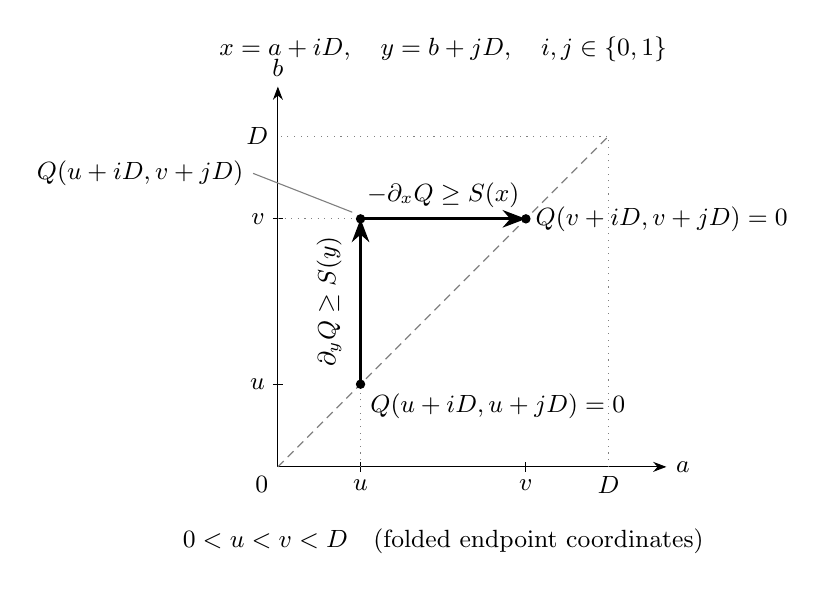
\begin{tikzpicture}[x=1.05cm,y=1.05cm,>=Stealth,font=\small]
  \draw[->] (0,0)--(4.7,0) node[right] {$a$};
  \draw[->] (0,0)--(0,4.6) node[above] {$b$};
  \draw[gray,densely dashed] (0,0)--(4,4);
  \draw[gray,dotted] (4,0)--(4,4)--(0,4);
  \node[below left] at (0,0) {$0$};
  \node[below] at (4,0) {$D$};
  \node[left] at (0,4) {$D$};
  \foreach \a/\b in {1/u,3/v} {
    \draw (\a,-.06)--(\a,.06) node[below=3pt] {$\b$};
    \draw (-.06,\a)--(.06,\a) node[left=3pt] {$\b$};
  }
  \draw[gray,dotted] (1,0)--(1,1);
  \draw[gray,dotted] (0,3)--(1,3);
  \draw[very thick,->] (1,1)--(1,3);
  \draw[very thick,->] (1,3)--(3,3);
  \fill (1,1) circle (1.7pt);
  \fill (1,3) circle (1.7pt);
  \fill (3,3) circle (1.7pt);
  \node[below right] at (1,1) {$Q(u+iD,u+jD)=0$};
  \node[anchor=east] (qtarget) at (-.3,3.55)
    {$Q(u+iD,v+jD)$};
  \draw[gray,thin] (qtarget.east)--(.9,3.08);
  \node[right,align=left] at (3,3) {$Q(v+iD,v+jD)=0$};
  \node[rotate=90,above] at (.89,2) {$\partial_yQ\ge S(y)$};
  \node[above] at (2,3.02) {$-\partial_xQ\ge S(x)$};
  \node[align=center] at (2,5.05)
    {$x=a+iD,\quad y=b+jD,\quad i,j\in\{0,1\}$};
  \node[align=center] at (2,-.9)
    {$0<u<v<D$\quad (folded endpoint coordinates)};
\end{tikzpicture}

\caption{The two paths in folded endpoint coordinates
$x=a+iD$, $y=b+jD$, for $0<u<v<D$.
The first starts at $Q=0$ and increases the second endpoint;
the second increases the first endpoint toward another zero.
The zeros come from the diagonal when $i=j$ and from the cut-pair
identity otherwise. Each moving endpoint stays in one open
half-period. When $i=1,j=0$, the actual order is $u+D>v$,
and both positive-semidefinite lower bounds still apply.}
\label{fig:schur-endpoint-paths}
\end{figure}

Both moving endpoints stay in one open half-period, so neither path
passes through a chart pole.  In particular, when $i=1,j=0$ the actual
endpoint order is $u+D>v$.  The first path starts at $(u+D,u)$ and the
second ends at $(v+D,v)$; the same zero values and the same derivative
inequalities apply.  Thus neither matrix inequality reverses in this
case.  Finally, the integrals on their right sides are positive
definite, so $Q(u+iD,v+jD)>0$.
\end{proof}

\subsection{Scalar lower bounds for the two factors}

For distinct $x,y\in\mathcal I$, define
\begin{equation}
 f_H(x,y)=
 \frac{|\det(H(y)-H(x))|}
 {\sqrt{\det H'(x)\det H'(y)}},\qquad
 f_K(x,y)=
 \frac{|\det Q(x,y)|}
 {\sqrt{\det S(x)\det S(y)}}.
 \label{eq:lag-two-factors}
\end{equation}
These auxiliary factors are symmetric under exchanging the actual
endpoints.  Combining \eqref{eq:lag-graph-determinant},
\eqref{eq:lag-velocity-factorization}, and
\eqref{eq:lag-Schur-factorization} gives
\begin{equation}
 f(x,y)=f_H(x,y)f_K(x,y).
 \label{eq:lag-factorization}
\end{equation}
The factors are positive away from the cut pairs $|y-x|=D$; at those
pairs $f_K=0$.

\begin{proposition}[Scalar block bounds]
\label{lag:block-bounds}
With the profiles of Proposition~\ref{lag:profiles}, every pair of
distinct chart endpoints satisfies
\begin{equation}
 f_H(x,y)^{1/m}\ge
 \frac{\left|\int_x^y h(t)\,dt\right|}{\sqrt{h(x)h(y)}}.
 \label{eq:lag-H-scalar-bound}
\end{equation}
For $0<u<v<D$ and $i,j\in\{0,1\}$ one has
\begin{equation}
 f_K(u+iD,v+jD)^{1/k}\ge
 \frac{
  \left(\int_u^v s_i(t)\,dt\right)^{1/2}
  \left(\int_u^v s_j(t)\,dt\right)^{1/2}}
 {\sqrt{s_i(u)s_j(v)}}.
 \label{eq:lag-K-scalar-bound}
\end{equation}
Together with endpoint exchange, these bounds cover the full square
$(0,T)^2$ except the chart, diagonal, and cut lines, a set of planar
measure zero.
\end{proposition}

\begin{proof}
We first record the determinant inequality used in both blocks.  For
a positive definite $r\times r$ matrix $M$, write
$\delta_r(M)=\det(M)^{1/r}$.  The elementary variational formula
\begin{equation}
 \delta_r(M)=
 \inf_{\substack{P>0\\\det P=1}}\frac1r\tr(PM)
 \label{eq:lag-determinant-variational}
\end{equation}
follows by applying the arithmetic--geometric mean inequality to the
eigenvalues of $M^{1/2}PM^{1/2}$.  Equality is attained at
$P=\delta_r(M)M^{-1}$.  The formula proves monotonicity under the
positive-semidefinite order.  It also proves, for any continuous
positive definite matrix function on a compact interval,
\begin{equation}
 \delta_r\left(\int_a^b M(t)\,dt\right)
 \ge\int_a^b\delta_r(M(t))\,dt.
 \label{eq:lag-Minkowski}
\end{equation}
Indeed, for every admissible $P$ the integral of
$\tr(PM(t))/r$ is at least the right side, and one then takes the
infimum over $P$.  This is the integral form of Minkowski's determinant
inequality; it retains the degree-one homogeneity of the determinant
root.

Apply \eqref{eq:lag-Minkowski} to $H'$ on the interval between $x$ and
$y$.  Equation~\eqref{eq:lag-H-difference} gives
\[
 |\det(\Delta H)|^{1/m}
 \ge\left|\int_x^y\det(H'(t))^{1/m}\,dt\right|.
\]
For $y<x$ this uses the positive matrix $-\Delta H$.  Division by
\[
 \bigl(\det H'(x)\det H'(y)\bigr)^{1/(2m)}
 =\sqrt{h(x)h(y)}
\]
proves \eqref{eq:lag-H-scalar-bound}.

Now put $Q=Q(u+iD,v+jD)>0$.  Each of the two matrix bounds in
Proposition~\ref{lag:schur}, followed by determinant monotonicity and
\eqref{eq:lag-Minkowski}, gives
\[
 \delta_k(Q)\ge\int_u^v s_i(t)\,dt,
 \qquad
 \delta_k(Q)\ge\int_u^v s_j(t)\,dt.
\]
Thus $\delta_k(Q)$ dominates their maximum and therefore their
geometric mean.  The denominator in the $k$th root of $f_K$ is exactly
\[
 \bigl(\det S(u+iD)\det S(v+jD)\bigr)^{1/(2k)}
 =\sqrt{s_i(u)s_j(v)},
\]
which proves \eqref{eq:lag-K-scalar-bound} with the displayed powers.

Finally, every endpoint in $\mathcal I$ has a unique expression
$u+iD$ with $0<u<D$ and $i\in\{0,1\}$.  For a pair whose folded
parameters differ, order those parameters as $u<v$, exchanging the
actual endpoints if necessary.  The preceding bounds apply for every
choice of the two half-period indices.  Equal folded parameters mean
either a diagonal pair or a cut pair.  The remaining excluded pairs
have an endpoint at $D$.  These are finitely many lines, and symmetry
of both factors justifies the endpoint exchange everywhere else.
\end{proof}

The two determinant roots have now been compared with scalar interval
integrals.  Proposition~\ref{lag:profiles} supplies exactly their
endpoint control.  The next section combines these bounds by a weighted
logarithmic identity.

\section{Weighted comparison along a closed geodesic}
\label{weighted:section}

We retain $D=\pi/2$, $T=\pi$, $d=n-1$, and $m=d-k$, with
$m,k\geq1$. The factorization $f=f_Hf_K$ turns the logarithm of
the ratio to the model density into a sum of two block contributions.
We will show that each contribution has nonnegative integral with
weight $w(|y-x|)$. The scalar identity below cancels the integrated
endpoint terms in the block bounds. A strict-convexity remainder
will then give the determinant comparison and identify its equality
case, without separately classifying equality in the matrix estimates.

The scalar identity is a logarithmic form of the weighted cancellation
in Kazdan's proof of the Berger--Kazdan inequality
\citep[Appendix~E, especially E.4--E.8]{Kazdan1978AppendixE}.
At interval length $\pi$, writing Kazdan's profile as
$\phi(t)=\sin(t)e^{u(t)}$ gives $p=\phi^{-2}$,
$p_0(t)=\sin^{-2}t$, $g=\log(p/p_0)=-2u$, and weight
$\rho(t)=W(t)/\sin t$.
We give the version needed here, with bounded logarithmic ratios
and a measurable weight, including the endpoint integrability.
Its application to the two factors depends on the folded symmetry
proved below.

\begin{lemma}[Weighted scalar identity]\label{weighted:scalar}
Let $b>0$, $\lambda=\pi/b$, and
\[
 p_0(t)=\frac{\lambda^2}{\sin^2(\lambda t)},\qquad 0<t<b.
\]
Let $p:(0,b)\to(0,\infty)$ be continuous and suppose that
$g=\log(p/p_0)$ is bounded.  Let $W$ be nonnegative and measurable on
$(0,b)$, with $W(b-z)=W(z)$ almost everywhere and
$W(z)/\sin(\lambda z)$ essentially bounded.  Write
\[
 \Delta_b=\{(x,y):0<x<y<b\},\qquad
 d\nu_{xy}(t)=\frac{p_0(t)\,dt}{\int_x^y p_0},\quad x<t<y.
\]
Then all the following integrals are finite, and
\begin{align}
 &\int_{\Delta_b}W(y-x)
 \left[\log\frac{\int_x^y p}{\int_x^y p_0}
       -\frac{g(x)+g(y)}2\right]dx\,dy \notag\\
 &\qquad=\int_{\Delta_b}W(y-x)
 \left[\log\int_x^y e^{g(t)}\,d\nu_{xy}(t)
       -\int_x^y g(t)\,d\nu_{xy}(t)\right]dx\,dy
 \ \geq\ 0.\label{weighted:scalar-identity}
\end{align}
\end{lemma}

\begin{proof}
Direct integration gives
\begin{equation}
 P_0(x,y):=\int_x^y p_0
 =\frac{\lambda\sin(\lambda(y-x))}
        {\sin(\lambda x)\sin(\lambda y)},\qquad
 \frac{P_0(x,y)}{\sqrt{p_0(x)p_0(y)}}
 =\frac{\sin(\lambda(y-x))}{\lambda}.
 \label{weighted:chord}
\end{equation}
The measure $\nu_{xy}$ is a probability measure.  Both its average of
$g$ and $\log\int e^g\,d\nu_{xy}=\log(\int p/\int p_0)$ have absolute
value at most $\|g\|_\infty$.  Since $W$ is essentially bounded, the asserted
finiteness follows already from these bounds.  Jensen's inequality makes
the integrand on the second line of
\eqref{weighted:scalar-identity} nonnegative.  It remains to establish
the equality of the integrated linear terms.

Set $K(z)=W(z)/\sin(\lambda z)$ and $I_W=\int_0^b W(z)\,dz$, and define
\[
 F(t)=\int_{0<x<t<y<b}
 K(y-x)\sin(\lambda x)\sin(\lambda y)\,dx\,dy.
\]
Here the two-variable kernel
$q(x,y)=K(y-x)\sin(\lambda x)\sin(\lambda y)$ is essentially bounded.
Fubini gives
\[
 F(t)=\int_0^t\left(\int_x^b q(x,y)\,dy\right)dx
       -\int_0^t\left(\int_0^y q(x,y)\,dx\right)dy.
\]
Thus $F$ is absolutely continuous on $[0,b]$, $F(0)=0$, and, for almost
every $t$,
\begin{align*}
 F'(t)
 &=\sin(\lambda t)\left[
   \int_0^{b-t}K(z)\sin(\lambda(t+z))\,dz
   -\int_0^t K(z)\sin(\lambda(t-z))\,dz\right]\\
 &=\sin(\lambda t)\int_0^b K(z)\sin(\lambda(t+z))\,dz\\
 &=I_W\sin(\lambda t)\cos(\lambda t).
\end{align*}
For the second equality substitute $b-z$ in the subtracted integral:
$K(b-z)=K(z)$ and
$\sin(\lambda(t-b+z))=-\sin(\lambda(t+z))$.
For the last equality, symmetry gives
$\int_0^b K(z)\cos(\lambda z)\,dz=0$, while
$\int_0^b K(z)\sin(\lambda z)\,dz=I_W$.
Integration therefore yields
\begin{equation}
 F(t)=\frac{I_W}{2\lambda}\sin^2(\lambda t),\qquad
 \frac{p_0(t)}{\lambda}F(t)=\frac{I_W}{2}.
 \label{weighted:coefficient}
\end{equation}
This argument has not differentiated the measurable weight.

Using \eqref{weighted:chord} and then
\eqref{weighted:coefficient}, the integrated interval averages are
\begin{align*}
 \int_{\Delta_b}W(y-x)\int_x^y g(t)\,d\nu_{xy}(t)\,dx\,dy
 &=\int_0^b g(t)\frac{p_0(t)}{\lambda}F(t)\,dt\\
 &=\frac{I_W}{2}\int_0^b g(t)\,dt.
\end{align*}
The exchange is absolutely integrable: replacing $g$ by $|g|$ in the
left side bounds it by
$\|g\|_\infty\int_{\Delta_b}W(y-x)\,dx\,dy$.
In particular, no integral of $p_0$ over the entire interval is taken.
The endpoint terms have exactly the same value, since
\begin{align*}
 &\frac12\int_{\Delta_b}W(y-x)(g(x)+g(y))\,dx\,dy\\
 &\qquad=\frac12\int_0^b g(t)
 \left[\int_0^{b-t}W(z)\,dz+\int_0^t W(z)\,dz\right]dt
 =\frac{I_W}{2}\int_0^b g(t)\,dt.
\end{align*}
The final equality again uses $W(b-z)=W(z)$.  Subtracting these equal
finite quantities proves the identity and hence the lemma.
\end{proof}

\begin{theorem}[Comparison on each geodesic]\label{weighted:geodesic}
In the normalized intermediate case of Proposition~\ref{geom:structure},
let $f(x,y)$ be the Jacobi determinant of any fixed unit-speed geodesic,
as in Proposition~\ref{lag:determinant}.  Put
\[
 \mathcal R=(0,T)^2,\qquad
 w(z)=(\sin z)^m\left|\frac{\sin(2z)}2\right|^k
 \quad(0\leq z\leq T).
\]
Then
\begin{equation}
 \int_{\mathcal R}f(x,y)\,dx\,dy
 \ \geq\ \int_{\mathcal R}w(|y-x|)\,dx\,dy.
 \label{weighted:comparison}
\end{equation}
Equality holds if and only if
$f(x,y)=w(|y-x|)$ for every $(x,y)\in[0,T]^2$.
\end{theorem}

\begin{proof}
All constants in this proof may depend on the chosen geodesic.
Write $w_{xy}=w(|y-x|)$.  We first work off the null set
\[
 E=\{(x,y)\in\mathcal R:
       x=D\text{ or }y=D\text{ or }x=y\text{ or }|y-x|=D\}.
\]
There $f,w_{xy}$, and the two determinant factors $f_H,f_K$ of
Proposition~\ref{lag:block-bounds} are positive, and $f=f_Hf_K$.  Define
\[
 L_H(x,y)=\log\frac{f_H(x,y)}{\sin^m(|y-x|)},\qquad
 L_K(x,y)=\log\frac{f_K(x,y)}{|\sin(2|y-x|)/2|^k}.
\]
Set their values on $E$ equal to zero for integration.
Both are symmetric in the actual endpoint slots $x,y$.

\paragraph{Finiteness of the logarithmic integrals.}
The profile bounds in Proposition~\ref{lag:profiles} give constants
$0<\alpha\leq\beta<\infty$ such that
\begin{align*}
 \alpha&\leq\frac{h(t)}{\csc^2t}\leq\beta
 &&(0<t<T),\\
 \alpha&\leq\frac{s_i(t)}{4\csc^2(2t)}\leq\beta
 &&(0<t<D,\ i=0,1).
\end{align*}
Set $\eta=\alpha/\beta\leq1$.
For $x<y$, the first bound in Proposition~\ref{lag:block-bounds} and the chord
identity \eqref{weighted:chord} imply
\[
 f_H(x,y)^{1/m}
 \geq\frac{\int_x^y h}{\sqrt{h(x)h(y)}}
 \geq\eta\sin(y-x).
\]
Symmetry gives this lower bound for either endpoint order.
Similarly, put $B_0(z)=\sin(2z)/2$ for $0<z<D$.
For $0<u<v<D$ and $i,j\in\{0,1\}$, the second block bound gives
\[
 f_K(u+iD,v+jD)^{1/k}
 \geq\frac{(\int_u^v s_i)^{1/2}(\int_u^v s_j)^{1/2}}
              {\sqrt{s_i(u)s_j(v)}}
 \geq\eta B_0(v-u).
\]
In these coordinates
$B_0(v-u)=|\sin(2|y-x|)/2|$.  Every pair outside $E$ has this form,
possibly after exchanging endpoints.  Consequently
\begin{equation}
 L_H\geq m\log\eta,
 \qquad L_K\geq k\log\eta,
 \qquad L_H+L_K=L:=\log(f/w_{xy}).
 \label{weighted:log-lower-bounds}
\end{equation}
With $a^+=\max(a,0)$, the elementary estimate
\[
 w_{xy}L^+\leq f
\]
and continuity of $f$ on the compact square prove integrability of
$w_{xy}L^+$.  The individual negative parts are bounded by
\eqref{weighted:log-lower-bounds}; also
\[
 L_H^+\leq L^+-k\log\eta,\qquad
 L_K^+\leq L^+-m\log\eta.
\]
Thus $w_{xy}L_H$, $w_{xy}L_K$, and $w_{xy}L$ are all absolutely
integrable.  The following additions of logarithmic integrals therefore
involve only finite quantities.

\paragraph{The $H$ factor on the full square.}
Apply Lemma~\ref{weighted:scalar} with
$b=T$, $\lambda=1$, $p=h$, and $W=w$.  Its assumptions hold by
Proposition~\ref{lag:profiles} and
\[
 w(T-z)=w(z),\qquad
 \frac{w(z)}{\sin z}
 =\sin^{m-1}z\left|\frac{\sin(2z)}2\right|^k,
\]
which is bounded because $m\geq1$.
Writing $g_H=\log(h/\csc^2t)$, the first block bound and
\eqref{weighted:chord} give, for $0<x<y<T$ outside $E$,
\[
 \frac{L_H(x,y)}m
 \geq\log\frac{\int_x^y h(t)\,dt}{\int_x^y\csc^2t\,dt}
       -\frac{g_H(x)+g_H(y)}2.
\]
After multiplication by $w(y-x)$, Lemma~\ref{weighted:scalar}
makes the integral of the right side nonnegative.  Multiplication by
$m$ and endpoint symmetry then yield
\begin{equation}
 \int_{\mathcal R}w_{xy}L_H(x,y)\,dx\,dy\geq0.
 \label{weighted:H-log}
\end{equation}

\paragraph{The $K$ factor and the four folded weights.}
Put $p_0(t)=4\csc^2(2t)$ on $(0,D)$ and define
\[
 g_i(t)=\log\frac{s_i(t)}{p_0(t)},\qquad
 A_i(u,v)=\log\frac{\int_u^v s_i(t)\,dt}{\int_u^v p_0(t)\,dt}
 \quad(i=0,1).
\]
For $(u,v)\in\Delta_D$, $z=v-u$, $x=u+iD$, and $y=v+jD$, the second
block bound gives the precise logarithmic inequality
\begin{equation}
 \frac{L_K(u+iD,v+jD)}k
 \geq\frac12\bigl[A_i(u,v)+A_j(u,v)-g_i(u)-g_j(v)\bigr].
 \label{weighted:folded-bound}
\end{equation}
Indeed, \eqref{weighted:chord} with $\lambda=2$ converts the reference
interval integral and its endpoint factors into $B_0(z)$.
The actual separation is $z$ if $i=j$, $D+z$ if $(i,j)=(0,1)$,
and $D-z$ if $(i,j)=(1,0)$.  In the last case $x>y$; the bound in
Proposition~\ref{lag:block-bounds} includes this order.
All three separations have the same absolute fast model factor
$B_0(z)$.

The four weights $w_{ij}(z)=w(|z+(j-i)D|)$ form the matrix
\begin{equation}
 (w_{ij}(z))_{i,j=0}^1
 =B_0(z)^k
 \begin{pmatrix}
  \sin^m z&\cos^m z\\
  \cos^m z&\sin^m z
 \end{pmatrix}.
 \label{weighted:weight-matrix}
\end{equation}
Every row and every column sums to
\[
 W_D(z)=(\sin^m z+\cos^m z)B_0(z)^k.
\]
This is symmetric under $z\mapsto D-z$, and
\[
 \frac{W_D(z)}{\sin(2z)}
 =2^{-k}(\sin^m z+\cos^m z)\sin^{k-1}(2z)
\]
is bounded for every $k\geq1$.  When $k=1$, its limit at either endpoint
is $1/2$, so this case also satisfies Lemma~\ref{weighted:scalar}.

Multiply \eqref{weighted:folded-bound} by $w_{ij}(z)$ and sum over
$i,j$.  The row sums control the terms indexed by $i$, and the column
sums control those indexed by $j$, giving exactly
\begin{align}
 \sum_{i,j=0}^1 w_{ij}(z)\frac{L_K(u+iD,v+jD)}k
 &\geq W_D(z)\sum_{i=0}^1
 \left[A_i(u,v)-\frac{g_i(u)+g_i(v)}2\right].
 \label{weighted:folded-sum}
\end{align}
Lemma~\ref{weighted:scalar}, applied on $(0,D)$ separately to $s_0$
and $s_1$ with weight $W_D$, shows that the right side has nonnegative
integral over $\Delta_D$.

For completeness, the four images of $\Delta_D$ used above consist
precisely of pairs whose first endpoint has smaller residue modulo $D$
than the second.  Their transposes contain precisely the opposite
residue order.  These eight disjoint regions cover $\mathcal R\setminus E$;
each coordinate change has Jacobian one.  Since $w_{xy}L_K(x,y)$ is
symmetric, it follows that
\begin{align}
 &\int_{\mathcal R}w_{xy}L_K(x,y)\,dx\,dy\notag\\
 &\qquad=2k\int_{\Delta_D}\sum_{i,j=0}^1
 w_{ij}(v-u)\frac{L_K(u+iD,v+jD)}k\,du\,dv
 \ \geq\ 0.
 \label{weighted:K-log}
\end{align}
Here the factor $2$ accounts for endpoint exchange and the factor $k$
restores the logarithm of $f_K$ from that of its $k$th root.

\paragraph{Comparison and equality.}
Adding \eqref{weighted:H-log} and \eqref{weighted:K-log} gives
\[
 \int_{\mathcal R}w_{xy}\log(f/w_{xy})\,dx\,dy\geq0.
\]
For $r>0$, the strictly convex function
\[
 \Phi(r)=r-1-\log r
\]
is nonnegative and vanishes exactly at $r=1$.  On
$\mathcal R\setminus E$ put $r=f/w_{xy}$.  All terms in the identity
\begin{equation}
 \int_{\mathcal R}(f-w_{xy})\,dx\,dy
 =\int_{\mathcal R}w_{xy}\log r\,dx\,dy
  +\int_{\mathcal R}w_{xy}\Phi(r)\,dx\,dy
 \label{weighted:strict-gap}
\end{equation}
are finite by the preceding integrability argument.  Both terms on
the right are nonnegative, proving \eqref{weighted:comparison}.
If equality holds, the last integral is zero.  Since $w_{xy}>0$ off
the diagonal and cut lines, $\Phi(r)=0$ almost everywhere, hence
$f=w_{xy}$ almost everywhere in $\mathcal R$.
Continuity of both functions on $[0,T]^2$ extends this identity to
every pair, including the exceptional lines and boundary.  Conversely,
that pointwise identity gives equality in \eqref{weighted:comparison}.
\end{proof}

\section{Global comparison and the equality case}
\label{rig:section}

We retain all intermediate model types and the normalization of
Section~\ref{geom:section}. The preceding geodesic comparison
now gives the global volume bound. Its nonnegative defect will
also retain enough information to identify the equality metric.

For $\xi\in U$, write $\gamma_\xi$ for the geodesic with initial
velocity $\xi$ and $f_\xi$ for the determinant of
Proposition~\ref{lag:determinant}. Put
\[
 J(\xi,t)=f_\xi(0,t).
\]
This is the absolute determinant of the normal Jacobi tensor
with initial value zero and derivative $\Id$. It is continuous
in $(\xi,t)$, positive for $0<t<D$, and agrees there with the
usual polar volume density.

\begin{lemma}[Polar integration over a full period]
\label{rig:polar}
For every $p\in M$,
\[
 \int_{S_pM}\int_0^D J(\xi,t)\,dt\,d\sigma_p(\xi)=V,
 \qquad
 \int_{S_pM}\int_0^T J(\xi,t)\,dt\,d\sigma_p(\xi)=2V.
\]
\end{lemma}

\begin{proof}
The open injectivity ball maps diffeomorphically onto the
complement of the cut locus. The latter is a smooth submanifold
of dimension $d-k<n$, hence has zero Riemannian volume.
Polar coordinates therefore prove the first formula.
Periodicity of the Jacobi data and reversal of the geodesic give
\[
 J(\xi,T-t)=J(\xi,-t)=J(-\xi,t).
\]
The sign in the reversed initial derivative disappears under the
absolute determinant. The substitution $t\mapsto T-t$ in the
second half-period, followed by the area-preserving antipodal
map on $S_pM$, proves the second formula.
\end{proof}

\begin{proof}[Proof of Theorem~\ref{thm:comparison}]
The circle, sphere-type, and real-projective-type cases are
already covered in Section~\ref{geom:section}. In an intermediate
case use the normalization \eqref{geom:normalization}.
Theorem~\ref{weighted:geodesic} says that
\begin{equation}\label{rig:geodesic-defect}
 \delta(\xi):=\int_0^T\int_0^T
   \bigl(f_\xi(x,y)-w(|y-x|)\bigr)\,dx\,dy\ge0.
\end{equation}
Time translation along a geodesic gives
\[
 f_\xi(x,y)=J\bigl(\phi_x\xi,(y-x)\bmod T\bigr).
\]
The possible choice of endpoint for the residue modulo $T$ has
no effect on any integral. Fubini's theorem, translation on the
time circle, flow invariance of $\mu$, and
Lemma~\ref{rig:polar} yield
\begin{align*}
 \int_U\int_0^T\int_0^T f_\xi(x,y)\,dx\,dy\,d\mu(\xi)
 &=T\int_U\int_0^T J(\xi,t)\,dt\,d\mu(\xi)\\
 &=2TV^2.
\end{align*}
All integrands are continuous and bounded on the compact
domains in question. Since $w(T-t)=w(t)$, its periodic
extension gives likewise
\begin{align*}
 \int_U\int_0^T\int_0^T w(|y-x|)\,dx\,dy\,d\mu(\xi)
 &=\sigma_d V T\int_0^T w(t)\,dt\\
 &=2TVV_0.
\end{align*}
Integrating \eqref{rig:geodesic-defect} and dividing by $2TV>0$
proves $V\ge V_0$.

If $V=V_0$, the nonnegative function $\delta$ has integral zero.
It is continuous, because the underlying Jacobi tensors depend
smoothly on the initial velocity and taking the absolute
determinant preserves continuity. Full support of $\mu$ forces
$\delta(\xi)=0$ for every $\xi$. The equality assertion in
Theorem~\ref{weighted:geodesic} now gives
\begin{equation}\label{rig:radial-density}
 J(\xi,t)=w(t),\qquad \xi\in U,\quad 0<t<D.
\end{equation}

In Cartesian normal coordinates at any point, the volume
density is $J(\xi,t)/t^d$. By \eqref{rig:radial-density} it depends
only on $t$. At the origin it extends smoothly with value one,
as also follows directly from the normal-coordinate volume
form. Thus $M$ is harmonic. It is compact and simply connected
by Proposition~\ref{geom:structure}. The compact simply
connected case of the Lichnerowicz conjecture, proved by
\citet{Szabo1990}, identifies its metric with a compact rank-one
symmetric metric up to scale. Its type identifies the model,
and the fixed diameter identifies the scale.
For the radial-density definition and the concluding metric
classification, see also the author's original preprint
\citep[pp.~2--4 and Lemmas~4.9--4.10]{Szabo1988}.

Conversely, a model is isometric to itself and has volume $V_0$.
Finally both sides of the volume comparison scale by the same
factor under a constant metric rescaling. Undoing
\eqref{geom:normalization} proves the assertion at every diameter.
\end{proof}

\begin{proof}[Proof of Corollary~\ref{thm:volume-reduction}]
The upper bound and Theorem~\ref{thm:comparison} give equal
volumes, so its equality case applies.
\end{proof}


\section{Incidence and the quaternionic Pontryagin class}
\label{inc:section}

The lower-volume comparison and its metric equality case are now
proved. To obtain the quaternionic upper bound, we first determine
the characteristic class of an actual bundle supplied by the cut
geometry: the normal four-plane bundle of cut incidence.
The later loop-energy construction will use this same bundle,
not only its sphere-fibration homotopy type.
We use the standard integral bundle and cohomology tools in
\citet{Hatcher2002} and \citet{MilnorStasheff1974}; the geometric
constructions and the relations needed here are proved below.
In this section and the next three, suppose that $M$ has quaternionic
type, so $n=4r$, $r\ge2$, and $k=3$. Choose an integral generator
$u\in H^4(M;\Z)$ and an orientation with $\int_Mu^r=1$.
Write $C_p=\operatorname{Cut}(p)$. The cell attachment in
Section~\ref{geom:section} gives
\[
 H^*(C_p;\Z)=\Z[u|_{C_p}]/((u|_{C_p})^r).
\]
Indeed restriction is an isomorphism in every degree below $4r-1$,
and $C_p$ has dimension $4r-4$. In particular it is orientable,
and its fundamental class is dual to $\pm u$ in $M$.

\subsection{The actual normal bundle}

\begin{proposition}\label{inc:normal}
The cut incidence
\[
 F=\{(p,q)\in M\times M:q\in C_p\}
\]
is a smooth embedded submanifold. Both projections are smooth
fiber bundles with fiber a cut locus. If $u_1,u_2$ are the two
pullbacks of $u$, its rank-four normal bundle $\mathcal V$ can be oriented
so that
\begin{equation}\label{inc:normal-classes}
 e(\mathcal V)=u_1-u_2,\qquad p_1(\mathcal V)=2s(u_1+u_2),\qquad s\in2\Z+1.
\end{equation}
Projection of $\mathcal V_{(p,q)}$ into $T_pM$ identifies it with
$N_pC_q$. The unit sphere of this four-plane is exactly the
great sphere of initial directions of minimizing geodesics
from $p$ to $q$.
\end{proposition}

\begin{proof}
The full cut map
\[
 c:SM\longrightarrow M\times M,\qquad
 c(\xi)=(\pi(\xi),\exp_{\pi(\xi)}(D\xi))
\]
has constant rank $4r+(4r-4)=8r-4$. Its fibers are the connected
great three-spheres from Proposition~\ref{geom:structure}.
Here constant rank and compactness give an embedded image,
as follows. Constant-rank charts give local image germs through
any image point. Charts overlapping along its fiber have the
same germ, so connectedness of that fiber makes all these germs
agree. Cover the compact fiber by finitely many such charts.
Properness excludes additional inverse images outside their
union over a sufficiently small neighborhood of the image point.
Thus the whole image in that neighborhood is the one smooth
submanifold germ. This proves the assertion. The first projection
is a submersion because its composition with $c$ is $\pi$;
symmetry gives the same conclusion for the second. Proper
submersions are smooth fiber bundles.

For $(a,b)\in \mathcal V_{(p,q)}\subset T_pM\oplus T_qM$, orthogonality
to $(T_pC_q,0)$ gives $a\in N_pC_q$. If $a=0$, surjectivity
of the second projection on $T_{(p,q)}F$ forces $b=0$.
The projection to $N_pC_q$ is therefore injective and, both
spaces having dimension four, an isomorphism. First variation
for the constant distance $D$ shows that the initial directions
from $p$ to $q$ are normal to $C_q$. Their great sphere has
the full dimension of $S(N_pC_q)$, proving the last assertion.
In particular, if $q_1,q_2\in C_p$ are distinct, then
\begin{equation}\label{inc:disjoint-planes}
 N_pC_{q_1}\cap N_pC_{q_2}=\{0\}:
\end{equation}
a common nonzero direction would reach both points at time $D$.

The cut loci and $M$ are simply connected, so the fibration
makes $F$ simply connected. Its normal bundle is orientable.
Leray--Hirsch \citep[Theorem~4D.1]{Hatcher2002}, using
$1,u_2,\ldots,u_2^{r-1}$ on the fibers,
and disjointness from the diagonal give the integral presentation
\begin{equation}\label{inc:ring}
 H^*(F;\Z)=\Z[u_1,u_2]/(u_1^{r+1},\Delta(u_1,u_2)),
 \qquad \Delta(a,b)=\sum_{j=0}^r a^jb^{r-j}.
\end{equation}
To justify completeness, the displayed relation is the restriction
of the diagonal class in $M\times M$. It is monic of degree $r$
in $u_2$, so the proposed quotient has exactly the Leray--Hirsch
basis. The dual of $F$ in $M\times M$ restricts on either factor
slice to $\pm u$. Its restriction to the disjoint diagonal is
zero. Its two factor coefficients are consequently opposite,
and after an orientation choice its restriction to $F$ is $u_1-u_2$.
The self-intersection formula gives the asserted Euler class.

The interchange of factors preserves the unoriented normal
bundle. Since $u_1,u_2$ are an integral basis of $H^4(F;\Z)$,
we have $p_1(\mathcal V)=t(u_1+u_2)$ for an integer $t$.
Also $H^2(F;\Z/2)=0$, so $\mathcal V$ is spin.
We use the classical identification
$\operatorname{Spin}(4)=\operatorname{SU}(2)\times\operatorname{SU}(2)$
and its two complex two-dimensional half-spin representations;
see \citet[Sections~2.1--2.2]{Moore2010}. For an oriented spin
four-plane bundle, its two complex half-spin bundles have
second Chern classes
\[
 \frac{-p_1(\mathcal V)+2e(\mathcal V)}4,\qquad
 \frac{-p_1(\mathcal V)-2e(\mathcal V)}4.
\]
This follows directly from the formal half-spin weights
$\pm(t_1+t_2)/2$ and $\pm(t_1-t_2)/2$, where
$p_1=t_1^2+t_2^2$ and $e=t_1t_2$.
Integrality in the basis $u_1,u_2$ implies $t\equiv2\pmod4$.
Writing $t=2s$ proves the proposition.
\end{proof}

Changing $u$ to $-u$ replaces $s$ by $-s$. Reverse the orientation
of $\mathcal V$ at the same time to retain
$e(\mathcal V)=u_1-u_2$, and reverse the orientation of $M$
exactly when $r$ is odd to retain $\int_Mu^r=1$.
We may therefore take $s\ge1$.

\subsection{The rank constraint from two direction planes}

For distinct $q_1,q_2\in C_p$, \eqref{inc:disjoint-planes} places
two four-planes with zero intersection inside $T_pM$. Their direct
sum has a complement of rank $4(r-2)$, which limits the degree
of its total Pontryagin class. We will use this rank restriction
to determine $p(TM)$ from $s$. The parameter space must therefore
exclude coincident cut points; put
\[
 Z=\{(p,q_1,q_2):q_1,q_2\in C_p,\ q_1\ne q_2\}.
\]
Use $v,x_1,x_2$ for the pullbacks of $u$ from its three points.
In this section polynomial degree is one quarter of cohomological
degree. In degrees divisible by four the rational cohomology of
$Z$ is the algebra
\begin{equation}\label{inc:triple-ring}
 A=\mathbb Q[v,x_1,x_2]/(v^{r+1},\Delta(v,x_1),S(v,x_1,x_2)),
 \quad
 S(v,x_1,x_2)=\sum_{i+j+\ell=r-1}v^ix_1^jx_2^\ell.
\end{equation}
Here and below this assertion identifies the subalgebra consisting
of these degrees; no claim about other degrees is needed.

For completeness, before removing $q_1=q_2$, Leray--Hirsch gives
the relations $v^{r+1}$, $\Delta(v,x_1)$ and $\Delta(v,x_2)$.
The relative diagonal has codimension $4(r-1)$. Its dual is
$\pm S$. To see this, the dual is a homogeneous polynomial of
degree $r-1$ annihilated by $x_1-x_2$. In degree $r$ the only
relations are the two displayed $\Delta$ polynomials; their
difference is $(x_1-x_2)S$. More explicitly, multiplying a
representative of the dual by $x_1-x_2$ gives a constant linear
combination of those two relations. Setting $x_1=x_2$ makes
the two constants opposite. Cancellation of $x_1-x_2$ then
takes place in the ordinary polynomial ring, before passage
to cohomology, and shows that the dual is proportional to $S$.
Restriction to a fixed-$p$ fiber gives the ordinary diagonal
class of $C_p\times C_p$, fixing the factor as $\pm1$.
The Thom sequence for removing the relative diagonal is
surjective onto the complement in degrees divisible by four,
because the relevant next cohomology group of $F$ is zero.
Restriction from the ambient fiber product to that diagonal is
surjective, so the projection formula identifies the kernel
with the ideal of its dual. The relation $\Delta(v,x_2)$ then
becomes redundant, proving \eqref{inc:triple-ring}.
Successive division by its two monic relations proves that $A$
is free over $\mathbb Q[v]/(v^{r+1})$, with basis
\begin{equation}\label{inc:free-basis}
 \{x_1^a x_2^b:0\le a<r,\ 0\le b<r-1\}.
\end{equation}

\begin{theorem}\label{inc:pontryagin}
The total Pontryagin class of $M$ is
\begin{equation}\label{inc:pontryagin-formula}
 p(TM)=\frac{(1+2su+u^2)^{r+1}}{1+4su}
 \quad\text{in }H^*(M;\mathbb Q).
\end{equation}
The quotient means its power-series expansion truncated by
$u^{r+1}=0$.
\end{theorem}

\begin{proof}
Over $Z$, the two actual normal four-planes in
\eqref{inc:disjoint-planes} have direct sum inside the pullback
of $TM$ from $p$. Choose a complementary bundle $W$ of rank
$4(r-2)$. Set
\[
 D_s(v,x)=1+2s(v+x)+(v-x)^2,
 \qquad p_0(v)=\frac{(1+2sv+v^2)^{r+1}}{1+4sv}.
\]
The rank-four identity $p_2=e^2$
\citep[Corollary~15.8]{MilnorStasheff1974} and
Proposition~\ref{inc:normal} give
\begin{equation}\label{inc:complement}
 p(W)=\frac{p(TM)(v)}{D_s(v,x_1)D_s(v,x_2)}.
\end{equation}
Its polynomial degree is at most $t_0=2r-4$.

We will prove that the formal characteristic class
\[
 \mathcal W_0=\frac{p_0(v)}{D_s(v,x_1)D_s(v,x_2)}\in A
\]
has degree at most $t_0$ and a degree-$t_0$ component that is nonzero
modulo $v$. The freeness in
\eqref{inc:free-basis} will then show that any first discrepancy
between $p(TM)(v)$ and $p_0(v)$ violates the rank bound on $W$.
For the degree bound we use only the algebra
\eqref{inc:triple-ring}, without presuming the answer for $TM$.
Successive monic polynomial divisions factor
\[
 T^{r+1}=(T-v)(T-x_1)(T-x_2)
                   \prod_{j=4}^{r+1}(T-z_j)
\]
in an extension of $A$ obtained by adjoining roots of monic
polynomials. Give each root degree one; the monic relations
are homogeneous for this grading. Each adjoining algebra is
free with a basis containing $1$, so this extension is injective. The positive-degree
elementary symmetric functions of all $r+1$ roots vanish.
Consequently, the product of $D_s(v,z)$ over all these roots is
$(1+2sv+v^2)^{r+1}$. The factor at $z=v$ is $1+4sv$.
Dividing these constant-one series therefore gives
\[
 \mathcal W_0=\prod_{j=4}^{r+1}D_s(v,z_j).
\]
There are $r-2$ factors, each of degree at most two, as required.

We also need the top component $(\mathcal W_0)_{t_0}$ to be nonzero
modulo $v$. For $r=2$ it is $1$. For $r\ge3$, let
\[
 (1+2sx+x^2)^{-1}=\sum_{j\ge0}a_jx^j.
\]
The recursion $a_0=1$, $a_1=-2s$ and
$a_j=-2sa_{j-1}-a_{j-2}$ gives
\begin{equation}\label{inc:reciprocal-identity}
 a_j^2-a_{j-1}a_{j+1}=1\qquad(j\ge1).
\end{equation}
Indeed the left side is unchanged on replacing $j$ by $j-1$,
and its initial value is one. Modulo $v$ the algebra can also be
presented as
\[
 \mathbb Q[x_1,x_2]/
 \left(x_1^r,x_2^r,\sum_{j=0}^{r-1}x_1^jx_2^{r-1-j}\right).
\]
In degree $2r-4$ the surviving monomials after the first two
truncations are
\[
 x_1^{r-3}x_2^{r-1},\qquad
 x_1^{r-2}x_2^{r-2},\qquad x_1^{r-1}x_2^{r-3}.
\]
The remaining ideal gives exactly their sum as a relation:
multiplying its generator by any monomial of degree $r-3$
gives this same sum. Their coefficients in $\mathcal W_0$ are, in order,
$a_{r-3}a_{r-1},a_{r-2}^2,a_{r-3}a_{r-1}$.
Equation~\eqref{inc:reciprocal-identity} makes the middle
coefficient differ from either outside coefficient by one.
Thus the component modulo $v$ is the nonzero class of
$x_1^{r-2}x_2^{r-2}$, one of the monomials in
\eqref{inc:free-basis}.

Finally suppose that $p(TM)(v)/p_0(v)$ first differs from $1$
in degree $i$, where $1\le i\le r$. Write its first coefficient
as $b\ne0$. In degree $t_0+i$, modulo $v^{i+1}$,
\eqref{inc:complement} is $b v^i(\mathcal W_0)_{t_0}$.
This is nonzero by \eqref{inc:free-basis} and the preceding
calculation: in a free module over $\mathbb Q[v]/(v^{r+1})$,
a coefficient nonzero modulo $v$ remains nonzero after
multiplication by $v^i$, modulo $v^{i+1}$, for $i\le r$.
It contradicts the rank bound on $W$.
Therefore there is no such $i$, which proves the theorem.
\end{proof}

\section{The signature determines the incidence coefficient}
\label{sig:section}

The incidence construction has reduced the bundle calculation to
one odd integer $s$. The signature theorem determines it in every
quaternionic rank. The small ranks follow from exact coefficients;
a single contour estimate treats all larger ranks.

\begin{theorem}\label{sig:coefficient}
In Proposition~\ref{inc:normal}, $|s|=1$. In particular, the
actual tautological four-plane bundle of every tangent great-sphere
fibration at a point of $M$ satisfies $p_1=\pm2e$.
\end{theorem}

\begin{proof}
Keep the choices $s\ge1$ and $\int_Mu^r=1$. Set
\[
 a_+a_-=1,\qquad a_+^2+a_-^2=2s,\qquad
 a_+\ge a_->0,\qquad c=2\sqrt{s},
 \quad f(y)=\frac{\sqrt y}{\tanh\sqrt y}.
\]
Hirzebruch's signature theorem
\citep[Signature Theorem~19.4]{MilnorStasheff1974}, applied to
Theorem~\ref{inc:pontryagin} gives
\begin{equation}\label{sig:formula}
 \sigma_r=[u^r]
 \frac{(f(a_+^2u)f(a_-^2u))^{r+1}}{f(c^2u)}.
\end{equation}
Here $f$ is its power series at zero; the two factors reflect
$1+2su+u^2=(1+a_+^2u)(1+a_-^2u)$.
The integral cohomology ring of $M$ gives
\[
 \sigma_r=\begin{cases}1,&r\text{ even},\\0,&r\text{ odd}.
 \end{cases}
\]
Indeed for even $r$ the middle pairing has the positive basis
$u^{r/2}$, and for odd $r$ its middle cohomology is zero.
Expanding $f(y)=1+y/3-y^2/45+2y^3/945+\cdots$ in
\eqref{sig:formula} gives
\[
 \sigma_2-1=\frac{8(s^2-1)}{15},\qquad
 \sigma_3=-\frac{32s(s^2-1)}{105}.
\]
These prove the assertion for $r=2,3$.

We give uniform estimates for all $r\ge4$. Since $s$ is odd,
the contrary case is $s\ge3$. We express the signature as a residue
and show that the two nearest nonzero poles give a main term that
dominates the remaining contour integral, forcing
$(-1)^r\sigma_r>1$. Put
\[
 \tau=\frac{a_-}{a_+}=s-\sqrt{s^2-1},\qquad
 b=\frac c{a_+}=\sqrt{2(1+\tau^2)},\qquad
 Q(z)=\tan z\tan(\tau z),\qquad \rho=\frac\pi{2b}.
\]
Then $0<\tau\le3-\sqrt8<0.172$ and
$\sqrt2<b<1.435$.
Substitute $u=-t^2$ in \eqref{sig:formula}. Since
$f(-a^2t^2)=at/\tan(at)$ and $a_+a_-=1$, taking the
coefficient by a residue and then putting $z=a_+t$ gives
\begin{equation}\label{sig:residue}
 (-1)^r\sigma_r=
 \frac\tau b\operatorname*{Res}_{z=0}
 \frac{\tan(bz)}{Q(z)^{r+1}}\,dz.
\end{equation}
The change of variables contributes the factor
$1/(ca_+)=\tau/b$; this fixes the normalization of the residue.

\paragraph{Contour representation.}
Take the rectangle with vertical sides $\Re z=\pm X$,
$X=3\pi/4$, and horizontal sides $\Im z=\pm4$.
Apart from zero, the only poles of the integrand in this rectangle
are at $z=\pm\rho$. Zeros of $\tan z$ occur only at multiples
of $\pi$, zeros of $\tan(\tau z)$ only at multiples of
$\pi/\tau$, and the next poles of $\tan(bz)$ are outside
because $3\pi/(2b)>X$. The poles of $\tan z$ at $\pm\pi/2$
give zeros of the reciprocal denominator, not poles.
Both residues at $\pm\rho$ equal
$-b^{-1}Q(\rho)^{-r-1}$, with $Q(\rho)>0$.
The residue theorem therefore expresses \eqref{sig:residue} as
\begin{equation}\label{sig:main-term}
 (-1)^r\sigma_r=L+\mathcal E,\qquad
 L=\frac{2\tau}{b^2}Q(\rho)^{-r-1}.
\end{equation}
Symmetry of the four sides and the triangle inequality bound
$|\mathcal E|/L$ by the sum of
\begin{align}
 E_v&=\frac b\pi\int_0^4
  |\tan(b(X+iy))|
  \left(\frac{Q(\rho)}{|Q(X+iy)|}\right)^{r+1}\,dy,
  \label{sig:vertical}\\
 E_h&=\frac b\pi\int_0^X
  |\tan(b(x+4i))|
  \left(\frac{Q(\rho)}{|Q(x+4i)|}\right)^{r+1}\,dx.
  \label{sig:horizontal}
\end{align}

\paragraph{Uniform bounds.}
The same contour works for every $r\ge4$ once both boundary ratios
are bounded by constants below one: their fifth powers then control
every exponent $r+1\ge5$. We retain the $\tau$ dependence in the
numerator and denominator so these bounds remain uniform as
$\tau\downarrow0$. All finite decimals below
denote the exact indicated rational numbers. Using
$3.14<\pi<3.142$ gives
\[
 \rho<1.111,\qquad \tan\rho<2.022,\qquad
 \tau\rho<0.192,\qquad Q(\rho)<2.30\tau.
\]
For the last inequality, the increase of $\tan t/t$ and the
Taylor bounds on $[0,0.192]$ give $\tan t/t<1.013$,
and $2.022\cdot1.111\cdot1.013<2.30$.
The same monotonicity gives
\begin{equation}\label{sig:ratio}
 \frac{Q(\rho)}{\tan(\tau X)}
 \le\frac{\rho\tan\rho}{X}<0.955.
\end{equation}
On the vertical sides, $|\tan(X+iy)|=1$.
Also $\cos(2bX)\ge0$, since
$2bX=3b\pi/2\in(2\pi,5\pi/2)$, and hence
$|\tan(b(X+iy))|\le1$.
The elementary complex tangent identity gives
\begin{align*}
 \frac{|\tan(\tau(X+iy))|^2}{\tan^2(\tau X)}
 &=\frac{1+\sinh^2(\tau y)/\sin^2(\tau X)}
         {1+\sinh^2(\tau y)/\cos^2(\tau X)}\\
 &\ge 1+0.08y^2\qquad(0\le y\le4).
\end{align*}
For this last bound, the numerator is at least $1+y^2/X^2$,
whereas $\cos(\tau X)>0.917$ and
$\sinh(\tau y)\le1.082\tau y$ bound the denominator by
$1+Ay^2$ with $A=(1.082\cdot0.172/0.917)^2$.
The inequality follows from
$X^{-2}\ge A+0.08+16(0.08)A$.
Since $r+1\ge5$, \eqref{sig:ratio} now implies
\begin{align*}
 E_v
 &<\frac{1.435}{3.14}(0.955)^5
      \int_0^4(1+0.08y^2)^{-5/2}\,dy\\
 &<0.783.
\end{align*}
Here the integral equals
\[
 \frac{4(1+2\cdot0.08\cdot16/3)}{(1+0.08\cdot16)^{3/2}}
 <2.154.
\]

On a horizontal side the identity for the modulus of tangent
gives
\[
 |Q(x+4i)|\ge\tanh4\,\tanh(4\tau),\qquad
 |\tan(b(x+4i))|\le\coth(4b)<1.001.
\]
Since $\tau/\tanh(4\tau)$ is increasing,
\[
 \frac{Q(\rho)}{\tanh4\,\tanh(4\tau)}
 <\frac{2.30\cdot0.172}{0.999\cdot0.595}.
\]
Substitution in \eqref{sig:horizontal}, with $X/\pi=3/4$,
therefore gives
\[
 E_h<\frac{3\cdot1.435}{4}\,1.001
       \left(\frac{2.30\cdot0.172}{0.999\cdot0.595}\right)^5
 <0.142.
\]
The numerical trigonometric inequalities used here can be checked
without numerical approximation: use
\[
 \sin t\le t-t^3/6+t^5/120,\qquad
 \cos t\ge1-t^2/2+t^4/24-t^6/720
 \quad(0\le t\le1.111)
\]
for $\tan\rho$ and the smaller real arguments. For the
hyperbolic inequalities use
\[
 \frac{\sinh t}{t}\le1+\frac{t^2}{6}
       +\frac{t^4/120}{1-t^2/42}\quad(0\le t\le0.688).
\]
The first seven terms of the exponential series at $1.376$
give $\tanh(0.688)>0.595$, while $e^8>2000$ gives
$\tanh4>0.999$. The same bound and $b>\sqrt2$ imply
$\coth(4b)<1.001$.

Finally $Q(\rho)<2.30\tau<1$, so \eqref{sig:main-term}
and $r+1\ge5$ imply
\[
 L>\frac{\tau}{1+\tau^2}(2.30\tau)^{-5}
 \ge\frac{1}{(1+0.172^2)\,2.30^5\,0.172^4}>17.
\]
Combining these estimates yields
\[
 (-1)^r\sigma_r>(1-0.783-0.142)17=1.275>1,
\]
contradicting either possible cohomological signature. Thus $s=1$.
Restricting \eqref{inc:normal-classes} to a fixed-$p$ fiber
gives $e(\mathcal V)=-u_2$ and $p_1(\mathcal V)=2u_2$ there.
Proposition~\ref{inc:normal} identifies this restriction with
the actual tautological four-plane bundle, which proves the
last assertion as well.
\end{proof}

\section{The geodesic space and its integral classes}
\label{geo:section}

Throughout this section, $M$ has quaternionic model type, so that
\[
 n=4r,\qquad r\ge2,\qquad d=4r-1,\qquad k=3,
 \qquad H^*(M;\Z)=\Z[u]/(u^{r+1}),\quad |u|=4.
\]
We retain the normalization $D=\pi/2$ and $T=2D=\pi$.
Choose the sign of $u$ as permitted by Theorem~\ref{sig:coefficient},
so that the actual four-plane bundle $\mathcal V$ on cut incidence
$F$ satisfies
\begin{equation}\label{geo:incidence-input}
 p_1(\mathcal V)=2(u_1+u_2).
\end{equation}
Orient $M$ by $\int_Mu^r=1$.
Only the characteristic-class conclusion
\eqref{geo:incidence-input} and the bundle identification in
Proposition~\ref{inc:normal} are used from the incidence argument.

Let $U=SM$, let $\pi:U\to M$ be the unit tangent projection, and
write $z=\pi^*u$.  The prime period is $T$, so the action
\[
 (\R/\Z)\times U\longrightarrow U,
 \qquad (a,w)\longmapsto\phi_{Ta}(w)
\]
is free.  Its quotient and quotient map will be denoted by
\[
 B=U/S^1,\qquad \rho:U\longrightarrow B.
\]
Thus $B$ is the closed smooth manifold of oriented, unmarked
geodesics, of dimension $2n-2$.

\subsection{The contact normalization and the two Gysin sequences}

The contact calculation is the volume method for periodic geodesic
flows associated with Weinstein \citep{Weinstein1974}; we include
it to fix the period, Euler sign and angular-area factors exactly.
The ensuing integral Gysin sequences, universal coefficient theorem
and Poincar\'e duality are used in their standard forms
\citep{Hatcher2002,MilnorStasheff1974}.
Yang's complex-projective volume calculation also uses the Gysin
sequences of the unit-tangent sphere bundle and the geodesic-circle
bundle \citep[pp.~381--382]{Yang1991}.  Here the degree-four
generator leads to a different middle-degree lattice.

Let $\lambda$ be the unit tangent contact form,
\[
 \lambda_w(\zeta)=\langle w,d\pi_w\zeta\rangle.
\]
Its Reeb flow is the unit-speed geodesic flow.  Consequently
$\theta=\lambda/T$ is a connection for the above $\R/\Z$ action:
it is invariant and integrates to one on each orbit.  Its curvature
is the pullback of a symplectic form $\omega_B$ on $B$.
We fix the Euler-class sign convention by
\[
 \rho^*\omega_B=d\theta,\qquad e=[\omega_B]\in H^2(B;\Z),
\]
and give $B$ its symplectic orientation.

\begin{proposition}[Contact volume]\label{geo:contact}
With this orientation and Euler class,
\begin{equation}\label{geo:contact-formula}
 N:=\int_B e^{4r-1}
   =\frac{(4r-1)!\,|S^{4r-1}|\,\Vol(M)}{T^{4r}}>0.
\end{equation}
For the standard quaternionic model at the same diameter, this
number is
\begin{equation}\label{geo:model-number}
 N_0=\frac{1}{2r+1}\binom{4r}{2r}.
\end{equation}
\end{proposition}

\begin{proof}
Integration over the circle fibers gives
\[
 \int_Be^d
 =\int_U\theta\wedge(d\theta)^d
 =T^{-(d+1)}\int_U\lambda\wedge(d\lambda)^d,
\]
where $U$ has the orientation induced by the positive circle
direction and the chosen orientation of $B$.
To compute the last form as a density, use the connection splitting
of $T_wU$ into horizontal and vertical directions.  Choose an
orthonormal frame $(w,e_1,\ldots,e_d)$ at $\pi(w)$.
The contact form reads off the horizontal $w$ coordinate, and
$d\lambda$ pairs each horizontal $e_i$ coordinate with its vertical
$e_i$ coordinate, up to one common sign convention.
In the $d$-fold exterior power each pairing occurs once in each of
$d!$ orders.  Hence
\[
 \big|\lambda\wedge(d\lambda)^d\big|=d!\,d\mu,
\]
where $d\mu$ is base Riemannian volume times unit tangent sphere
area.  The chosen orientation makes the contact integral positive,
and $\mu(U)=|S^d|\Vol(M)$.  Since $d+1=4r$, this proves
\eqref{geo:contact-formula}.

The model's polar density on $(0,D)$ is
$\sin^{4r-1}t\cos^3t$.  With $y=\sin^2t$,
\[
 \int_0^{\pi/2}\sin^{4r-1}t\cos^3t\,dt
 =\frac12\int_0^1 y^{2r-1}(1-y)\,dy
 =\frac{1}{4r(2r+1)}.
\]
Using $|S^{4r-1}|=2\pi^{2r}/(2r-1)!$ and $T=\pi$ in
\eqref{geo:contact-formula} gives
\[
 N_0=\frac{(4r-1)!}{r(2r+1)((2r-1)!)^2}
     =\frac{(4r)!}{(2r)!(2r+1)!},
\]
which is \eqref{geo:model-number}.
\end{proof}

Thus the desired upper volume bound is $N\le N_0$.  The integral
cohomology calculation below computes the determinant of a middle
pairing whose entries are top-degree products, including this
characteristic number.

\begin{lemma}[Integral Gysin information]\label{geo:gysin}
The manifolds $U$ and $B$ are simply connected.  There is an
integral class $v\in H^4(B;\Z)$ with $\rho^*v=z$.
For $2j<n$, the following is an integral basis:
\begin{equation}\label{geo:low-basis}
 H^{2j}(B;\Z):\qquad
 e^{j-2a}v^a,\qquad 0\le a\le\lfloor j/2\rfloor.
\end{equation}
All odd cohomology of $B$ vanishes, and its even cohomology is free
abelian.  In particular $H^2(B;\Z)=\Z e$ and
$H^4(B;\Z)=\Z e^2\oplus\Z v$.
The rational cohomology ring is generated by $e,v$, and
\begin{equation}\label{geo:total-betti}
 \dim_{\mathbb Q}H^*(B;\mathbb Q)=2r(r+1).
\end{equation}

Multiplication by $e$ at the middle fits into an exact sequence
\begin{equation}\label{geo:middle-sequence}
 0\longrightarrow H^{n-2}(B;\Z)
 \xrightarrow{\ e\smile\ }H^n(B;\Z)
 \longrightarrow\Z/(r+1)\longrightarrow0.
\end{equation}
Consequently the integral bilinear form
\begin{equation}\label{geo:middle-form}
 (a,b)\longmapsto\int_B eab,\qquad a,b\in H^{n-2}(B;\Z),
\end{equation}
has determinant of absolute value $r+1$ in any integral basis.
The map $e\smile:H^n(B;\Z)\to H^{n+2}(B;\Z)$ is an
isomorphism.
\end{lemma}

\begin{proof}
The sphere fiber of $\pi$ has dimension $n-1\ge7$.  Its homotopy
sequence and simple connectivity of $M$ give $\pi_1(U)=0$.
The homotopy sequence of the circle bundle then gives $\pi_1(B)=0$.

The Euler number of $TM$ is $\chi(M)=r+1$.  The chosen orientation
therefore gives
\[
 e(TM)=(r+1)u^r.
\]
The integral Gysin sequence of the oriented sphere bundle $\pi$
has the form
\[
 H^{q-n}(M)\xrightarrow{\ e(TM)\smile\ }H^q(M)
 \xrightarrow{\ \pi^*\ }H^q(U)
 \xrightarrow{\ \pi_!\ }H^{q-n+1}(M)
 \xrightarrow{\ e(TM)\smile\ }H^{q+1}(M).
\]
It gives the complete additive calculation
\begin{equation}\label{geo:unit-cohomology}
 H^q(U;\Z)=
 \begin{cases}
  \Z\{z^a\},&q=4a,\quad 0\le a<r,\\
  \Z/(r+1)\{z^r\},&q=n,\\
  \Z\{y_a\},&q=n-1+4a,\quad 1\le a\le r,\\
  0,&\text{otherwise}.
 \end{cases}
\end{equation}
Here the upper generators may be chosen with
$\pi_!y_a=u^a$ and $y_a=z^{a-1}y_1$; the latter assertion follows
from the projection formula and the fact that $\pi_!$ is an
isomorphism in these upper degrees.
At degree $n-1$, the Gysin map from $H^0(M)$ to $H^n(M)$ is
multiplication by the nonzero integer $r+1$, so
$H^{n-1}(U)=0$.  This also explains the sole torsion group in
\eqref{geo:unit-cohomology}.

Apply next the integral Gysin sequence of $\rho$.  The vanishing
of odd groups of $U$ below degree $n$ inductively gives
$H^{2j-1}(B)=0$ for $2j-1<n$.  For positive even $2j<n$ the
remaining terms give
\begin{equation}\label{geo:low-exact}
 0\longrightarrow H^{2j-2}(B)
 \xrightarrow{\ e\smile\ }H^{2j}(B)
 \xrightarrow{\ \rho^*\ }H^{2j}(U)
 \longrightarrow0.
\end{equation}
For $2j=2$ this says $H^2(B)=\Z e$.  For $2j=4$, the last
group is freely generated by $z$, so choose an integral lift $v$.
If $j$ is odd, the last group in \eqref{geo:low-exact} vanishes
and multiplication by $e$ gives the next basis.  If $j=2a$ is
even, the last group is generated by $z^a$, and the class $v^a$
lifts that generator.  Induction proves exactly the integral basis
\eqref{geo:low-basis}.

In all degrees at most $n-2$, the homology groups of $B$ are free
and have the same ranks as its cohomology groups.  Indeed the
universal coefficient theorem detects torsion in $H_i(B;\Z)$
as torsion in $H^{i+1}(B;\Z)$, and the latter groups are free
through degree $n-1$.  Poincar\'e duality on the oriented
$(2n-2)$-manifold $B$ now supplies all its cohomology in degrees
at least $n$.  It is free in even degrees and zero in odd degrees;
together with the low-degree calculation this proves the asserted
global statement.

The circle Gysin sequence at degree $n$ uses
$H^{n-1}(U)=H^{n-1}(B)=0$ and
$H^n(U)=\Z/(r+1)$, and is precisely
\eqref{geo:middle-sequence}.  The Poincar\'e pairing
\[
 H^{n-2}(B;\Z)\times H^n(B;\Z)\longrightarrow\Z
\]
is unimodular, since these two groups are free.  Composing one
factor with the injection of index $r+1$ in
\eqref{geo:middle-sequence} proves the determinant assertion
\eqref{geo:middle-form}.
Finally $H^{n+1}(U)=H^{n+2}(U)=0$ by
\eqref{geo:unit-cohomology}.  The next portion of the circle
Gysin sequence therefore makes multiplication by $e$ from degree
$n$ to degree $n+2$ an isomorphism.

In every even degree $q\ge n$, the group $H^q(U;\mathbb Q)$
vanishes.  The rational circle Gysin sequence therefore makes
$e\smile:H^{q-2}(B;\mathbb Q)\to H^q(B;\mathbb Q)$
surjective.  The low-degree bases now show that the full rational
ring is generated by $e,v$.  Below degree $n$, the basis ranks
sum to
\[
 \sum_{j=0}^{2r-1}\bigl(\lfloor j/2\rfloor+1\bigr)
 =2\sum_{a=0}^{r-1}(a+1)=r(r+1).
\]
Poincar\'e duality supplies another $r(r+1)$ dimensions above
degree $n-1$, and the middle odd group is zero.  This proves
\eqref{geo:total-betti}.
\end{proof}

\subsection{The first free-loop attachment}

The Gysin sequences determine the low-degree integral lattice and its middle
determinant, but not the relations among $e$ and $v$.  Those
relations will come from the first nonconstant critical manifold
of the free-loop energy.

Write $\Lambda M=H^1(\R/T\Z,M)$ for the Sobolev free loop
space, with rotation of the parameter as its circle action.
The continuous-loop and Sobolev-loop models have the same homotopy
type, compatibly with evaluation and rotation.  We use the energy
\[
 \mathcal E(c)=\frac12\int_0^T|\dot c(t)|^2\,dt.
\]
For a circle space $A$, write $A_{hS^1}=ES^1\times_{S^1}A$.
The constant-loop subspace has trivial action, hence its Borel
construction is $M\times BS^1$.

\begin{proposition}[The first attachment and its coefficient]
\label{geo:attachment}
There is an oriented rank-three vector bundle $E\to B$ and an
attaching map
\[
 f:S(E)\longrightarrow M.
\]
Let $p:S(E)\to B$ and put $x=f^*u\in H^4(S(E);\Z)$.
The following properties hold:
\begin{enumerate}[label=\textup{(\roman*)}]
\item The pullback $\rho^*E$ is the first negative bundle for the
      free-loop energy.  It is isomorphic as a real vector bundle
      to the rank-three bundle $K\to U$ with fiber
      \[
       K_w=\{a\in w^\perp:
          J_a(D)=0\},
       \quad J_a(0)=0,\quad J_a'(0)=a,
      \]
      where $J_a$ is the normal Jacobi field along $\gamma_w$.
\item Let $\widetilde p:S(\rho^*E)\to U$ and
      $\widehat\rho:S(\rho^*E)\to S(E)$ be the pullback square.
      Then
      \begin{equation}\label{geo:attachment-pullback}
       \widehat\rho^*x=\widetilde p^*z.
      \end{equation}
\item After choosing the orientation of $E$, one has
      \begin{equation}\label{geo:primitive-boundary}
       p_!x=e.
      \end{equation}
      With either orientation its coefficient is $\pm1$.
\item The actual negative bundle satisfies
      \begin{equation}\label{geo:negative-pontryagin}
       \rho^*p_1(E)=4z.
      \end{equation}
\end{enumerate}
\end{proposition}

The attaching map makes $x^{r+1}=f^*(u^{r+1})=0$.
The sphere integral $p_!x=e$ fixes the coefficient of the fiber
part of $x$, while $\rho^*p_1(E)=4z$ carries the incidence
coefficient to the actual negative bundle.  Separating $x$ into
base and fiber parts will turn its nilpotence into relations on
$B$.  The middle determinant will then fix the scale of the
top-degree pairing used to evaluate $N$.

Figure~\ref{fig:attachment-pullback} distinguishes the pullback
square from the evaluation homotopy used in part~\textup{(ii)}.
\begin{figure}[tbp]
\centering
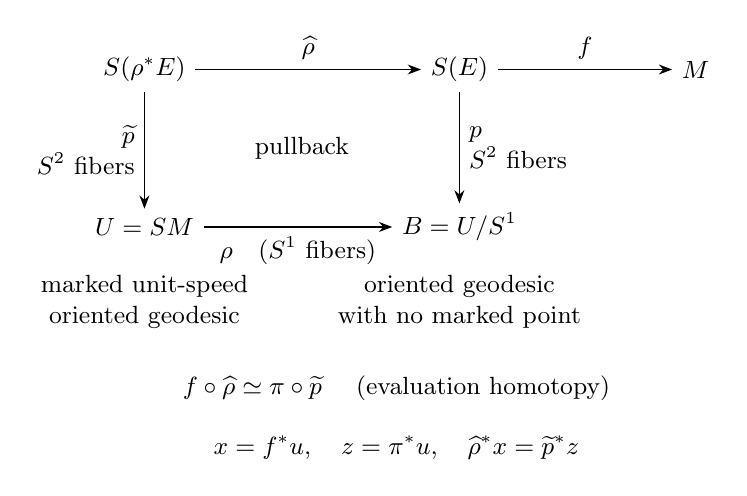
\begin{tikzpicture}[>=Stealth,font=\small]
  \node (SU) at (-3,1.8) {$S(\rho^*E)$};
  \node (SB) at (1,1.8) {$S(E)$};
  \node (U) at (-3,-.2) {$U=SM$};
  \node (B) at (1,-.2) {$B=U/S^1$};
  \node (M) at (4,1.8) {$M$};
  \draw[->] (SU)--node[above] {$\widehat\rho$} (SB);
  \draw[->] (SB)--node[above] {$f$} (M);
  \draw[->] (SU)--node[left,align=right] {$\widetilde p$\\$S^2\text{ fibers}$} (U);
  \draw[->] (SB)--node[right,align=left] {$p$\\$S^2\text{ fibers}$} (B);
  \draw[->] (U)--node[below] {$\rho\quad(S^1\text{ fibers})$} (B);
  \node[fill=white] at (-1,.8) {pullback};
  \node[align=center] at (-3,-1.15) {marked unit-speed\\oriented geodesic};
  \node[align=center] at (1,-1.15) {oriented geodesic\\with no marked point};
  \node[align=center] at (.2,-2.25)
    {$f\circ\widehat\rho\simeq\pi\circ\widetilde p$
      \quad (evaluation homotopy)};
  \node[align=center] at (.2,-3.0)
    {$x=f^*u,\quad z=\pi^*u,\quad
       \widehat\rho^*x=\widetilde p^*z$};
\end{tikzpicture}

\caption{The sphere bundle of the descended rank-three bundle $E$
and its pullback to $U=SM$. The square is a pullback, with vertical fibers
$S^2$ and horizontal fibers $S^1$. The attaching map $f$ is not
point evaluation of an unmarked geodesic. Evaluation of the
attachment gives the displayed homotopy and hence the equality
of cohomology classes.}
\label{fig:attachment-pullback}
\end{figure}

\begin{proof}
We give the index, attachment, and integral-coefficient details.

\paragraph{Critical manifolds and indices.}
The positive critical levels are $j^2T/2$, $j\ge1$; the critical
manifold at each is a copy of $U$, parametrized by
$w\mapsto(t\mapsto\gamma_w(jt))$.  These are all the nonconstant
critical loops because every geodesic has prime length $T$.

For the $j$th iterate, reparametrize variations by arclength on
$[0,jT]$.  The kernel of the periodic Hessian consists of all
periodic Jacobi fields.  All normal Jacobi fields are $T$-periodic
by the differential of $\phi_T=\Id$, so their dimension is $2d$.
A tangential Jacobi field is an affine scalar multiple of the
velocity; the periodic boundary conditions force its scalar to be
constant.  The kernel therefore has dimension $2d+1=\dim U$.
Variations of the initial unit tangent vector, including the
time-shift direction, realize precisely these fields.
Thus the Hessian kernel is the
tangent space to the critical manifold, as required by the
Morse--Bott condition.

The periodic index equals the fixed-endpoint index.  To see this
without an index correction formula, evaluation at the marked
initial point maps the periodic kernel onto $T_{\pi(w)}M$:
arbitrary normal initial values are possible, and the constant
tangent field supplies the remaining direction.  Choose a linear
right inverse to this evaluation.  Subtracting the corresponding
kernel field from a periodic test field makes both endpoint
values zero.  The index form is unchanged, including its mixed
terms, because a kernel field pairs to zero with every periodic
test field by integration by parts.  This subtraction is injective
on every negative definite subspace.  Conversely, fixed-endpoint
test fields form a subspace of the periodic domain.  The two
indices are consequently equal.

Interior conjugate instants on $[0,jT]$ occur at the $j$ odd
multiples of $D$, with multiplicity three, and the $j-1$ positive
multiples of $T$, with multiplicity $d$.  The fixed-endpoint Morse
index theorem \citep[Theorem~15.1, p.~83]{Milnor1963} gives
\begin{equation}\label{geo:iterate-index}
 \lambda_j=3j+d(j-1).
\end{equation}
In particular $\lambda_1=3$, while every later index is at least
$d+6=n+5\ge13$. The index count is unchanged on completing the
piecewise smooth zero-endpoint fields in $H^1$: the index form
is continuous, and any finite negative Gram matrix remains
negative after sufficiently close smooth approximation.

\paragraph{Negative bundles and attachment.}
Let $\nu\to U$ be the negative spectral bundle of the periodic
$L^2$ Jacobi operator
\[
 \mathscr A_w V=-\nabla_t^2V-R(V,\dot\gamma_w)\dot\gamma_w.
\]
This self-adjoint operator has domain the periodic $H^2$ fields,
and its quadratic form is the index form on periodic $H^1$ fields.
Its negative eigenvalues form an isolated finite cluster. The
constant index and nullity, together with compactness of $U$,
make the corresponding spectral projections locally smooth in
the initial data. Elliptic regularity makes their eigenfields
smooth, so $\nu$ is a genuine rank-three bundle.
It represents the negative bundle for the Hilbert-space
Morse--Bott attachment as well. Indeed, projection from the
negative subspace of the bounded $H^1$-Riesz Hessian to $\nu_w$
is injective: a vector in its kernel would have nonnegative
index form in the $L^2$ spectral decomposition. Equal negative
ranks make this a bundle isomorphism.
Each fixed parameter rotation intertwines these operators and
projections with those at the rotated geodesic. The resulting
action on $\nu$ is continuous and covers the free smooth circle
action on $U$. Hence $\nu$ descends to a real bundle $E\to B$,
with $\nu\cong\rho^*E$. Since $B$ is simply connected, $E$ is
orientable.

We use the Morse--Bott disk-attachment theorem for the energy on
the $H^1$ loop space of a closed Riemannian manifold.  The energy
satisfies the Palais--Smale condition.  Its Hessian is nondegenerate
normal to each compact critical manifold just described, and has
finite negative index. The bounded $H^1$ Hessian is Fredholm;
its identified kernel therefore gives an invertible restriction
normal to the critical manifold, as in the formulation cited
below. Thus sublevels bracketing one critical
value differ, up to homotopy, by the disk and sphere bundles of
its negative bundle.  This construction also respects parameter
rotation.  Indeed each fixed rotation is a smooth isometry for
the natural loop-space metric, preserves energy, commutes with
the gradient deformation, and preserves the Hessian splitting.
The local normal form and the contraction of its positive
directions may be constructed from these invariant metrics and
splittings.  Joint differentiability of the circle action on the
whole $H^1$ manifold is not needed.  For this equivariant
negative-bundle formulation see \citet[Section~7, pp.~2190--2192]
{OttosenBokstedt2007}, following the Hilbert-space attachment of
\citet[Theorem~2.4.10]{Klingenberg1978}.
The associated Borel vector bundle and Thom quotient are described
in \citet[Lemma~5.1, pp.~2185--2186]{OttosenBokstedt2007}.

Here is the attaching map and its evaluation property explicitly.
Start a sufficiently small negative disk at every first-level
geodesic by pointwise exponential of the negative fields.  Its
boundary lies strictly below the first positive critical value,
uniformly over $U$.  That lower sublevel deforms equivariantly to
the constants.  This follows from the noncritical energy
deformation between the boundary level and a small positive
level, followed by contraction of small loops to constants.  For
the latter, embed $M$ in Euclidean space, average a sufficiently
short loop, and project the straight contraction to a tubular
neighborhood of $M$.  Small energy gives uniformly small length,
so this is defined and continuous, preserves the constants, and
commutes with rotation.  The projection has bounded derivative,
so choosing the initial small level sufficiently small keeps this
contraction below the first critical value.

Insert the boundary deformation in an outer collar of the small
negative disk bundle.  This produces an equivariant map of pairs
\[
 \mathcal F_1:(D(\nu),S(\nu))\longrightarrow(\Lambda M,M)
\]
whose zero section is the first critical manifold and which
represents its Morse--Bott attachment.  On the boundary it takes
values in the constants.  Because the action on the constants
is trivial, this boundary map descends to
$f:S(E)\to M$.  Evaluation at time zero composed with
$\mathcal F_1$ is homotopic, by radial contraction of the disk
fibers, to $\pi$ composed with their bundle projection.  Restrict
this homotopy to $S(\nu)\cong S(\rho^*E)$.  Its boundary value
is $f\circ\widehat\rho$, which proves
\eqref{geo:attachment-pullback}.

Choose regular sublevels $\Lambda_-$ and $\Lambda_+$ immediately
below and above the first positive critical value.  The preceding
attachment gives, over $\Z$ or any field $\mathbb F$,
\begin{align}
 H^q(\Lambda_+,M;\mathbb F)
     &\cong H^{q-3}(U;\mathbb F),
       \label{geo:ordinary-relative}\\
 H^q((\Lambda_+)_{hS^1},M\times BS^1;\mathbb F)
     &\cong H^{q-3}(B;\mathbb F).
       \label{geo:borel-relative}
\end{align}
These are Thom isomorphisms; in the second one the free first
critical action identifies the Borel negative bundle with $E$
up to homotopy.  One can take finite-dimensional free
approximations to $ES^1$ throughout, apply the invariant
attachment, and then pass to the limit.
For every later critical level, the Borel negative bundle still
exists over the Borel critical manifold even though the action
has finite stabilizers.  Its relative cohomology vanishes below
its rank $\lambda_j$, with any necessary orientation local
system.  The same statement holds without the Borel construction.
Equation~\eqref{geo:iterate-index} therefore shows that subsequent
attachments do not change cohomology in degrees at most five.
The exhaustion by sublevels causes no extra term in these degrees:
the restriction systems in the relevant degrees are eventually
constant, so their inverse-limit obstruction vanishes.

We have constructed the attachment and isolated the degrees in
which no later attachment can alter it. What remains is to fix
its coefficient integrally and identify its actual negative bundle.

\paragraph{The coefficient is a unit over every prime field.}
Since $H^2(B;\Z)=\Z e$, write $p_!x=c e$ with $c\in\Z$.
Under \eqref{geo:borel-relative}, the connecting homomorphism
\[
 H^4(M\times BS^1;\mathbb F)
 \longrightarrow
 H^5((\Lambda_+)_{hS^1},M\times BS^1;\mathbb F)
 \cong H^2(B;\mathbb F)
\]
sends the class $u$ from $M$ to $p_!x$, up to the Thom
orientation sign.  Indeed the connecting map first restricts
to the attaching sphere, where that class is $x$, and then
uses the boundary map for $(D(E),S(E))$; the inverse Thom
isomorphism identifies this last map with integration over the
oriented sphere fiber.

Suppose that $c$ vanished modulo a prime $\ell$, and put
$\mathbb F=\Z/\ell$.  Exactness would extend the pure class
$u\in H^4(M\times BS^1;\mathbb F)$ over
$(\Lambda_+)_{hS^1}$ and hence over $(\Lambda M)_{hS^1}$,
by the higher-index gap.  After forgetting equivariance, its
restriction would be the evaluation class
\[
 a=\operatorname{ev}_0^*u\in H^4(\Lambda M;\mathbb F).
\]
To justify uniqueness here, \eqref{geo:ordinary-relative} gives
$H^4(\Lambda_+,M;\mathbb F)=H^1(U;\mathbb F)=0$.
Higher attachments have no effect in this range, so restriction
$H^4(\Lambda M;\mathbb F)\to H^4(M;\mathbb F)$ is injective.
The evaluation class is already one extension of $u$, and thus
is the only one.

An ordinary class restricted from the Borel construction has
zero action slant.  For completeness, if $Y$ is any circle space,
fix $e_0\in ES^1$ and let $i(y)=[e_0,y]\in Y_{hS^1}$.
For the action map $A:S^1\times Y\to Y$, the two maps
$i\circ A$ and $i\circ\operatorname{pr}_Y$ are homotopic:
\[
 [e_0,gy]=[e_0g,y],
\]
and the loop $g\mapsto e_0g$ contracts in $ES^1$.
Consequently the pullback of a Borel class under $i\circ A$
has no component in
$H^1(S^1;\mathbb F)\otimes H^{*-1}(Y;\mathbb F)$.
Equivalently its slant with $[S^1]$ is zero.  This is also the
usual action description of the Borel $d_2$ differential.

The evaluation class $a$ has a nonzero action slant over every
prime field.  The integral cohomology ring of $M$ and the
universal coefficient theorem give $H_2(M;\Z)=H_3(M;\Z)=0$.
Simple connectivity and successive applications of the Hurewicz
theorem \citep[Theorem~4.32]{Hatcher2002} make $M$
three-connected; Hurewicz then identifies
$\pi_4(M)$ with $H_4(M;\Z)=\Z$.
Choose a based map $g:S^4\to M$ with
$\langle g^*u,[S^4]\rangle=1$, and let
$\widehat g:S^3\to\Omega M\subset\Lambda M$ be its adjoint.
Evaluation of the rotated based loops on $S^1\times S^3$
factors, up to the orientation convention, through the smash
quotient
\[
 S^1\times S^3\longrightarrow S^1\wedge S^3=S^4
 \xrightarrow{\ g\ }M.
\]
The quotient takes the cross-product fundamental class to the
fundamental class of $S^4$, up to sign.  Therefore
\[
 \left\langle\widehat g^*
       \big(A^*\operatorname{ev}_0^*u/[S^1]\big),[S^3]\right\rangle
 =\pm1
\]
integrally, and remains nonzero after reduction modulo $\ell$.
This contradicts the zero slant required of the hypothesized
Borel extension.  No prime divides $c$, so $c=\pm1$.
Reverse the orientation of $E$ if necessary to obtain
\eqref{geo:primitive-boundary}.

\paragraph{The negative bundle is the cut-fiber tangent bundle.}
For $a\in K_w$, truncate $J_a$ to the first half-period and
extend it by zero on the second half:
\[
 \widehat J_a(t)=
 \begin{cases}
 J_a(t),&0\le t\le D,\\
 0,&D\le t\le T.
 \end{cases}
\]
The endpoint values agree, so this is an $H^1$ periodic test
field.  Integration by parts on $[0,D]$, with the vanishing
endpoint values and the Jacobi equation, gives zero index form
on this entire three-dimensional space.  Project these fields
to the negative spectral space $\nu_w$.  If a projected vector
were zero, its zero index form and its membership in the
nonnegative spectral subspace would force it into the Hessian
kernel.  It would then be a smooth periodic Jacobi field.
But a nonzero $J_a$ has nonzero derivative at $D$, since both
zero value and zero derivative would make it identically zero.
Its truncation has a derivative jump at $D$ and cannot be a
kernel field.  The projection is thus injective, and equal ranks
make it an isomorphism $K_w\to\nu_w$.
The truncation depends continuously in the $H^1$ norm on $w$
and $a$, and the spectral projections vary continuously as
above.  We obtain an isomorphism of real bundles
$K\cong\nu\cong\rho^*E$.
The truncations are used in the $H^1$ form domain, not in the
$H^2$ operator domain; their derivative jump is the reason
that a nonzero truncation cannot lie in the smooth kernel.

Finally define the full cut map
\[
 \mathfrak a:U\longrightarrow F,
 \qquad \mathfrak a(w)=(\pi(w),\exp_{\pi(w)}(Dw)).
\]
By the actual bundle identification in
Proposition~\ref{inc:normal}, its pullback of $\mathcal V$
is the initial-direction four-plane.  The marked unit direction
$w$ gives a trivial line in this plane; its orthogonal complement
is exactly $K_w$, the tangent space of the great-three-sphere
fiber.  Hence
\[
 \mathfrak a^*\mathcal V\cong\R\oplus K
 \cong\R\oplus\rho^*E.
\]
The two point maps from $U$ to $M$ in $\mathfrak a$ are
$\pi$ and $\pi\circ\phi_D$.  The geodesic flow provides a
homotopy between them, so
$\mathfrak a^*u_1=\mathfrak a^*u_2=z$.
Taking first Pontryagin classes and using
\eqref{geo:incidence-input} proves
\eqref{geo:negative-pontryagin}.
\end{proof}

\subsection{Half-integral lifts and the middle pairing}

On each sphere fiber, half the Euler class of its tangent bundle
integrates to one.  This gives a normalized fiber class with which
to separate $x$ into base and fiber parts.  The base class may be
only half-integral; we will track its displacement from the integral
lift $v$ so that the middle determinant is preserved.

\begin{proposition}[Arithmetic parameters]\label{geo:parameters}
Let $p:S(E)\to B$ and $x$ be as in
Proposition~\ref{geo:attachment}, and let
\[
 \xi=\frac12e(T_{\mathrm{vert}}S(E))\in H^2(S(E);\mathbb Q),
 \qquad X=e^2\in H^4(B;\Z).
\]
There is a class $Y\in H^4(B;\mathbb Q)$ such that, with
pullbacks by $p$ suppressed,
\begin{equation}\label{geo:sphere-parameters}
 x=Y+e\xi,\qquad
 \xi^2=p_1(E)/4,\qquad p_!\xi=1,\qquad
 \rho^*Y=z,\qquad 2Y\in H^4(B;\Z).
\end{equation}
For an integer $b$,
\begin{equation}\label{geo:Y-lift}
 Y=v+\frac b2e^2.
\end{equation}
There are rational numbers $\alpha,\beta$ with
\begin{equation}\label{geo:L-parameters}
 L:=e^2p_1(E)/4=\alpha X^2+\beta XY,\qquad
 4\alpha\in\Z,\qquad |\beta|=1.
\end{equation}
Here $\beta=1$ for \eqref{geo:incidence-input}; retaining $\beta$
also allows the opposite generator convention, for which
$\beta=-1$.
Moreover
\begin{equation}\label{geo:two-nilpotents}
 (Y+e\xi)^{r+1}=(Y-e\xi)^{r+1}=0
 \quad\text{in }H^*(S(E);\mathbb Q).
\end{equation}

Count $X,Y$ as polynomial degree one, corresponding to
cohomological degree four.  For homogeneous polynomials of
degree $2r-1$, set
\[
 \ell(P)=\int_B eP(X,Y).
\]
Then the middle moment matrix satisfies
\begin{equation}\label{geo:moment-determinant}
 \left|\det\left[
 \ell\big(X^{2r-1-i-j}Y^{i+j}\big)
 \right]_{0\le i,j<r}\right|=r+1,
 \qquad \ell(X^{2r-1})=N.
\end{equation}
Pullback $p^*:H^*(B;\mathbb Q)\to H^*(S(E);\mathbb Q)$
is injective, and multiplication by $e$ on $H^n(B;\mathbb Q)$
is injective.
\end{proposition}

\begin{proof}
Give each unit sphere fiber the boundary orientation from $E$.
The marked unit vector in $p^*E$ spans a trivial line, with
orthogonal complement the oriented vertical tangent two-plane:
\[
 p^*E\cong\R\oplus T_{\mathrm{vert}}S(E).
\]
For an oriented real two-plane bundle, the first Pontryagin
class is the square of its Euler class.  Thus
$\xi^2=p^*p_1(E)/4$.  On a sphere fiber the Euler class of
its tangent bundle integrates to two, giving $p_!\xi=1$.

The Euler class of the oriented rank-three bundle $E$ lies in
$H^3(B;\Z)=0$, so it vanishes.  The sphere-bundle Gysin
sequence then gives, in every degree, a short exact sequence
whose first map is $p^*$ and whose last map is $p_!$.
In particular $p^*$ is injective.  Over $\mathbb Q$, the
classes $1,\xi$ restrict to a basis of each sphere's cohomology,
so Leray--Hirsch gives the module decomposition
\[
 H^*(S(E);\mathbb Q)
 =p^*H^*(B;\mathbb Q)
  \oplus\xi\,p^*H^{*-2}(B;\mathbb Q).
\]
Since $p_!x=e$, there is a unique rational class $Y$ with
$x=p^*Y+p^*e\,\xi$.
The integral class
\[
 2x-p^*e\,e(T_{\mathrm{vert}}S(E))
\]
has zero sphere integral.  Integral Gysin exactness expresses
it as $p^*Y_2$ for $Y_2\in H^4(B;\Z)$.  Rational injectivity
of $p^*$ gives $Y_2=2Y$.  This proves half-integrality without
assuming that $Y$ itself is integral.

Pull back to the square over $U$ in
Proposition~\ref{geo:attachment}.  The class $\rho^*e$ vanishes,
as it does for the Euler class pulled to its own circle bundle.
Equation~\eqref{geo:attachment-pullback} now gives
\[
 \widetilde p^*(\rho^*Y)=\widehat\rho^*x
 =\widetilde p^*z.
\]
The pullback sphere bundle also has zero Euler class; its
rational Gysin sequence makes $\widetilde p^*$ injective.
It follows that $\rho^*Y=z$.
Write $2Y=a v+b e^2$ in the integral basis supplied by
Lemma~\ref{geo:gysin}.  Since $\rho^*v=z$ is a primitive
generator of $H^4(U;\Z)$, pulling back gives $a=2$.
This proves \eqref{geo:Y-lift}.

Similarly, integrality of $p_1(E)$ and
\eqref{geo:negative-pontryagin} give
\[
 p_1(E)=A e^2+4v,\qquad A\in\Z.
\]
If the opposite sign of the incidence coefficient is retained,
this reads $p_1(E)=A e^2+4\beta v$, with $\beta=\pm1$.
In either convention substitution of
$v=Y-(b/2)e^2$ gives
\[
 L=\frac{A-2\beta b}{4}X^2+\beta XY.
\]
Thus $4\alpha=A-2\beta b$ is integral, proving
\eqref{geo:L-parameters}.

The first equality in \eqref{geo:two-nilpotents} is
$x^{r+1}=f^*(u^{r+1})=0$.  Fiber antipodal reflection covers
the identity of $B$ and reverses the orientation of the
two-dimensional sphere fibers.  Its pullback fixes base classes
and sends the vertical Euler class, hence $\xi$, to its negative.
Pulling back the first equality proves the second one.

It remains to identify the moment determinant.  An integral
basis of $H^{n-2}(B;\Z)$ from
\eqref{geo:low-basis} is
\[
 b_i=eX^{r-1-i}v^i,\qquad 0\le i<r.
\]
The matrix of \eqref{geo:middle-form} in this basis has entries
\[
 \int_Be b_i b_j
 =\int_B eX^{2r-1-i-j}v^{i+j}.
\]
Replace $v$ in these basis vectors by
$Y=v+(b/2)X$.  The change of basis over $\mathbb Q$ is triangular
with every diagonal entry equal to one.  Hence its determinant
is one and it does not change the determinant of the bilinear
form.  Lemma~\ref{geo:gysin} proves the first assertion in
\eqref{geo:moment-determinant}.  The second follows from
$eX^{2r-1}=e^{4r-1}$ and the definition of $N$.
The final injectivity statements were proved above for $p^*$
and in Lemma~\ref{geo:gysin} for multiplication by $e$.
\end{proof}

\section{The sharp quaternionic volume bound}
\label{alg:section}

We retain the notation of Section~\ref{geo:section}.  Thus $n=4r$,
$r\ge2$, and
\[
 X=e^2,\qquad L=e^2p_1(E)/4=\alpha X^2+\beta XY,
 \qquad 4\alpha\in\Z,\quad |\beta|=1.
\]
In this section the polynomial degrees of $X$ and $Y$ are both one;
one polynomial degree therefore means cohomological degree four.
Let
\begin{equation}
 \ell(P)=\int_{B} eP(X,Y),
 \qquad \deg P=2r-1.
 \label{alg:functional}
\end{equation}
The inputs of Proposition~\ref{geo:parameters} include
\begin{equation}
 I_j=\ell(X^{2r-1-j}Y^j),\qquad
 \left|\det(I_{i+j})_{0\le i,j<r}\right|=r+1,
 \qquad N=I_0>0.
 \label{alg:middle-input}
\end{equation}
Our goal is
$N\le\binom{4r}{2r}/(2r+1)$, the model value computed in
Proposition~\ref{geo:contact}. The attachment gives polynomial
relations; the middle determinant fixes the scale of the top
functional; an explicit coefficient sum then gives the bound.
We do not prescribe the cohomology ring of the geodesic quotient
in advance.

\subsection{The power relations and the nonzero parameter}

Introduce a formal variable $Z$ with $Z^2=L$ and define homogeneous
polynomials in $X,Y$ by
\begin{align}
 Q(X,Y)&=\frac{(Y+Z)^{r+1}-(Y-Z)^{r+1}}{2Z}
   =\sum_{j\ge0}\binom{r+1}{2j+1}Y^{r-2j}L^j,
   \label{alg:Q}\\
 R(X,Y)&=\frac{(Y+Z)^{r+1}+(Y-Z)^{r+1}}2
   =\sum_{j\ge0}\binom{r+1}{2j}Y^{r+1-2j}L^j.
   \label{alg:R}
\end{align}
Only the terms with valid binomial indices are included.  The quotient
in~\eqref{alg:Q} is a polynomial identity; it involves no division by a
cohomology class.  The degrees of $Q,R$ are $r,r+1$, respectively.

\begin{lemma}
\label{alg:relations}
The classes $Q(X,Y)$ and $R(X,Y)$ vanish in
$H^*(B;\mathbb Q)$.  Moreover $\alpha\ne0$, and consequently
$|4\alpha|\ge1$.
\end{lemma}

\begin{proof}
On the sphere bundle $p:S(E)\to B$, the attachment class is
$x=Y+e\xi$ and satisfies $x^{r+1}=0$.  The fiber antipode sends $\xi$
to $-\xi$, so $(Y-e\xi)^{r+1}=0$ as well.  Taking the sum gives
$p^*R=0$.  The rational Leray--Hirsch decomposition with basis $1,\xi$
makes $p^*$ injective, hence $R=0$.  Taking the difference and integrating
over the sphere fiber, using $p_!\xi=1$, gives $eQ=0$.  The class $Q$ has
cohomological degree $4r=n$, and multiplication by $e$ is injective from
$H^n(B;\mathbb Q)$ to $H^{n+2}(B;\mathbb Q)$ by
Lemma~\ref{geo:gysin}.  Therefore $Q=0$.

Suppose now that $\alpha=0$.  We use the nondegenerate moment pairing
in~\eqref{alg:middle-input} to obtain a contradiction.  Write
\[
 q(y)=Q(1,y),\qquad a(y)=R(1,y),\qquad
 A_0=\C[y]/(q).
\]
The polynomial $q$ has degree $r$ and leading coefficient $r+1$.
The relations $Q=0$ imply that the rule $y^j\mapsto I_j$, for
$0\le j\le2r-1$, agrees with reduction modulo $q$ followed by a
functional $F:A_0\to\C$.  Indeed, every multiple of $q$ needed in
dividing a polynomial of this degree has multiplier of degree at most
$r-1$, and its homogenization is a top-degree multiple of $Q$.
Thus the matrix of $(f,g)\mapsto F(fg)$ in $1,y,\ldots,y^{r-1}$ is
precisely the nonsingular matrix in~\eqref{alg:middle-input}.
The relation $R=0$ similarly gives
\begin{equation}
 F(a(y)y^j)=0\qquad(0\le j\le r-2).
 \label{alg:orthogonal-R}
\end{equation}

Let $\varepsilon:A_0\to\C$ extract the coefficient of $y^{r-1}$
in the remainder of degree less than $r$.  Its product pairing is
nondegenerate: the entry $\varepsilon(y^{i+j})$ is zero when
$i+j<r-1$ and one when $i+j=r-1$, for $0\le i,j<r$.
Reversing the columns gives a triangular matrix with diagonal entries one.
Hence there is a unique $b\in A_0$ such that
$F(f)=\varepsilon(bf)$ for all $f$.  Nondegeneracy of the $F$ pairing
means that multiplication by $b$ is invertible, so $b$ is a unit.
For the $\varepsilon$ pairing the orthogonal complement of
$1,y,\ldots,y^{r-2}$ consists exactly of the constants.  To see this,
write a remainder $c_0+\cdots+c_{r-1}y^{r-1}$ and successively test
against $1,y,\ldots,y^{r-2}$; the tests force
$c_{r-1},c_{r-2},\ldots,c_1$ to vanish in that order.
Equation~\eqref{alg:orthogonal-R} therefore says that $ba$ is constant.
In particular any nonzero class $a$ satisfying that equation must be a
unit: its product with the unit $b$ is a nonzero constant.

But the class of $a=R(1,y)$ is nonzero and is not a unit.  Both $q$ and
$a$ vanish at $y=0$ when $\alpha=0$, so evaluation at zero precludes
invertibility.  To check that the class is nonzero, choose an
$(r+1)$st root of unity $\eta\ne1,-1$, and put
\[
 c_\eta=\frac{\eta-1}{\eta+1},\qquad
 y_0=\frac{\beta}{c_\eta^2},\qquad Z_0=c_\eta y_0.
\]
These numbers are nonzero, $Z_0^2=\beta y_0$, and
$y_0+Z_0=\eta(y_0-Z_0)$ with $y_0-Z_0\ne0$.  The formulas for $Q,R$
give $q(y_0)=0$ but $a(y_0)=(y_0-Z_0)^{r+1}\ne0$.  Thus $a$ cannot
be zero modulo $q$, a contradiction.  We conclude that $\alpha\ne0$.
Its stated integrality then gives $|4\alpha|\ge1$.
\end{proof}

\begin{lemma}
\label{alg:complete-intersection}
For $\alpha\ne0$, the polynomials $Q,R$ have no common nonzero zero
over $\C$.  The algebra
\[
 \mathcal A=\C[X,Y]/(Q,R)
\]
has Hilbert series
\begin{equation}
 \frac{(1-t^r)(1-t^{r+1})}{(1-t)^2}
   =(1+t+\cdots+t^{r-1})(1+t+\cdots+t^r).
 \label{alg:hilbert}
\end{equation}
In particular its top degree is $2r-1$, with dimension one, and
\begin{equation}
 X:\mathcal A_{r-1}\longrightarrow\mathcal A_r
 \quad\hbox{is an isomorphism},\qquad
 \dim\mathcal A_{r-1}=\dim\mathcal A_r=r.
 \label{alg:middle-isomorphism}
\end{equation}
Furthermore the complete rational relation ideal of the classes
$e,Y$ is generated by $Q(e^2,Y)$ and $R(e^2,Y)$.
\end{lemma}

\begin{proof}
At a common zero $(X,Y)$ choose a complex square root $Z$ of
$\alpha X^2+\beta XY$.  If $Z\ne0$, simultaneous vanishing of $Q,R$
would force both $(Y+Z)^{r+1}$ and $(Y-Z)^{r+1}$ to vanish, which is
impossible unless $Y=Z=0$.  If $Z=0$, the formulas become
$Q=(r+1)Y^r$ and $R=Y^{r+1}$, so $Y=0$; then $\alpha X^2=0$
forces $X=0$ as well.

The two homogeneous polynomials are therefore relatively prime.
Multiplication by $Q$ in $\C[X,Y]$ is injective, and multiplication by
$R$ is injective modulo $Q$: in the polynomial unique factorization
domain, $Q\mid Rf$ and relative primality imply $Q\mid f$.
The two resulting multiplication exact sequences give
\eqref{alg:hilbert}.  On setting $X=0$, the quotient becomes
$\C[Y]/(Y^r)$.  Thus the degree-$r$ cokernel of multiplication by $X$
vanishes.  The two dimensions read from~\eqref{alg:hilbert} are equal,
which proves~\eqref{alg:middle-isomorphism}.

For the assertion about the whole cohomology ring,
Lemma~\ref{geo:gysin} gives generation of $H^*(B;\mathbb Q)$
by $e,v$ and total dimension $2r(r+1)$.
Since $Y=v+(b/2)e^2$ by \eqref{geo:Y-lift}, the same ring is
generated by $e,Y$.

The polynomial algebra $\C[e,Y]$ is free on $1,e$ over $\C[X,Y]$
under $X=e^2$.  Quotienting by the two displayed relations therefore
gives $\mathcal A\oplus e\mathcal A$, of dimension $2r(r+1)$ by
\eqref{alg:hilbert}.  Its surjection to $H^*(B;\C)$ is an
isomorphism by the equality of dimensions.  The relations and maps are
defined over $\mathbb Q$, giving the rational assertion as well.
\end{proof}

\subsection{An explicit top functional and its determinant}

The algebraic method is the classical perfect-pairing duality for
finite graded complete intersections; see
\citet[Corollary~3.5 and the discussion following Theorem~9.1]
{Huneke1999}.
We make the pairing explicit to determine its normalization and
the required determinant.

The power relations suggest replacing $Y+Z$ and $Y-Z$ by two nilpotent
variables $a_1,a_2$.  With $Y=(a_1+a_2)/2$ and $Z=(a_1-a_2)/2$,
the equation $Z^2=L$ becomes a quadratic relation for $X$.
The resulting algebra admits explicit coefficient extraction; the
involution exchanging $a_1,a_2$ will recover the pairing on $\mathcal A$
without cancelling $Z$.

For any complex $\alpha\ne0$ and any complex $\beta$, set
\begin{equation}
 \mathcal D_{\alpha,\beta}=
 \frac{\C[a_1,a_2,X]}
 {\bigl(a_1^{r+1},a_2^{r+1},
  4\alpha X^2+2\beta(a_1+a_2)X-(a_1-a_2)^2\bigr)}.
 \label{alg:extraction-algebra}
\end{equation}
All three variables have polynomial degree one.  Every class has a
unique remainder that has $X$-degree at most one and each $a_i$-degree
at most $r$.  Denote extraction of $Xa_1^ra_2^r$ in that remainder by
$\varepsilon_{\mathcal D}$.  On homogeneous polynomials of degree
$2r-1$ define
\begin{equation}
 \Phi_{\alpha,\beta}(P)=
 \varepsilon_{\mathcal D}\left(
   (a_1-a_2)^2P\left(X,\frac{a_1+a_2}{2}\right)\right).
 \label{alg:Phi}
\end{equation}

\begin{lemma}
\label{alg:determinant}
The functional $\Phi_{\alpha,\beta}$ descends to the top degree of
$\mathcal A$ and is nonzero.  If
\[
 J_j=\Phi_{\alpha,\beta}(X^{2r-1-j}Y^j),
\]
then for every $\alpha\ne0$ and every $\beta\in\C$,
\begin{equation}
 \det(J_{i+j})_{0\le i,j<r}
 =(-1)^{r(r+1)/2}(r+1)(4\alpha)^{-r(r-1)/2}.
 \label{alg:determinant-formula}
\end{equation}
For the geometric parameters there is consequently a scalar $K$ with
\begin{equation}
 \ell=K\Phi_{\alpha,\beta},\qquad
 |K|=|4\alpha|^{(r-1)/2}.
 \label{alg:normalization}
\end{equation}
\end{lemma}

\begin{proof}
Put $Y=(a_1+a_2)/2$ and $Z=(a_1-a_2)/2$ inside $\mathcal D$.
Its quadratic relation becomes $Z^2=L$ and its other relations become
\[
 R=0,\qquad ZQ=0.
\]
It follows at once that multiplying either $R$ or $Q$ by $4Z^2$ gives
zero, so~\eqref{alg:Phi} annihilates the top-degree multiples of both
relations.

We next prove nondegeneracy, uniformly in the complex parameter $\beta$.
The coefficient functional on
\[
 D_0=\C[a_1,a_2]/(a_1^{r+1},a_2^{r+1})
\]
extracting $a_1^ra_2^r$ has a perfect product pairing, since every
monomial pairs with its complementary monomial.  The quadratic relation
in~\eqref{alg:extraction-algebra} is monic after division by $4\alpha$,
so $\mathcal D=D_0\oplus XD_0$.  Its coefficient pairing is perfect as
well.  Indeed, if $f+Xg$ annihilates every element of $D_0$, extraction
shows that $g=0$; testing then against $XD_0$ shows that $f=0$.
The grading makes this a perfect pairing between complementary degrees
summing to $2r+1$.

The involution exchanging $a_1,a_2$ preserves
$\varepsilon_{\mathcal D}$.  Its even and odd subspaces are therefore
orthogonal, and the odd subspaces in complementary degrees pair
perfectly.  Their exact module description is particularly useful.
Before imposing $R,ZQ$, the relation $Z^2=L$ gives the direct sum
\[
 \C[X,Y]\oplus Z\C[X,Y].
\]
The ideal generated by $R,ZQ$ has even part $(R,LQ)$ and odd part
$Z(R,Q)$.  Consequently
\begin{equation}
 \mathcal D^-\simeq Z\mathcal A
 \quad\hbox{as a graded module, with a shift by one}.
 \label{alg:odd-module}
\end{equation}
This follows by taking the two summands of the ideal; no cancellation
of $Z$ in the quotient is used.

By~\eqref{alg:middle-isomorphism}, multiplication by $X$ carries
$\mathcal D^-_r$ isomorphically onto $\mathcal D^-_{r+1}$.
In the basis
\[
 (a_1-a_2)X^{r-1-i}Y^i,\qquad 0\le i<r,
\]
of $\mathcal D^-_r$, the bilinear pairing
$(f,g)\mapsto\varepsilon_{\mathcal D}(fXg)$ has matrix
$(J_{i+j})$.  It is nondegenerate because the odd complementary-degree
pairing is perfect.  This proves in particular that $\Phi$ is nonzero.

For fixed nonzero $\alpha$, reduction of powers of $X$ by its monic
quadratic relation makes every $J_j$ a polynomial in $\beta$.
The determinant is thus a polynomial in $\beta$ which, by the preceding
argument, has no complex zero.  It is a nonzero constant in $\beta$.
It remains to evaluate it at $\beta=0$.

First set $\alpha=1/4$ as well, so that $X^2=(a_1-a_2)^2$.
In $\mathcal A$ use the linear coordinates
\[
 A_1=Y+X/2,\qquad A_2=Y-X/2.
\]
For $p+q=2r-1$, the coefficient of $X$ in the quadratic remainder of
$A_1^pA_2^q$ is the polynomial
\[
 \frac{a_1^pa_2^q-a_1^qa_2^p}{2(a_1-a_2)}.
\]
The numerator is divisible by $a_1-a_2$.  Multiplying by
$(a_1-a_2)^2$ and extracting $a_1^ra_2^r$ gives
\begin{equation}
 \Phi_{1/4,0}(A_1^pA_2^q)=
 \begin{cases}
 -1,&(p,q)=(r,r-1),\\
 1,&(p,q)=(r-1,r),\\
 0,&\text{otherwise}.
 \end{cases}
 \label{alg:base-functional}
\end{equation}
In the degree-$(r-1)$ monomial basis
$A_1^{r-1-i}A_2^i$, the matrix of the middle $X=A_1-A_2$ pairing
has entries $-2$ for $i+j=r-1$, entries $1$ for $i+j=r-2$ or $r$,
and zero otherwise.  Reversing columns gives the tridiagonal matrix
with diagonal $-2$ and adjacent entries $1$.
Its size-$r$ determinant is $(-1)^r(r+1)$: expansion along the last
row gives the recurrence $d_r=-2d_{r-1}-d_{r-2}$ with $d_0=1,d_1=-2$.
Column reversal has sign $(-1)^{r(r-1)/2}$.
The linear change from $X,Y$ to $A_1,A_2$ has determinant one, so its
degree-$(r-1)$ monomial change also has determinant one.  We have proved
\eqref{alg:determinant-formula} at $(\alpha,\beta)=(1/4,0)$.

At $\beta=0$ for general $\alpha\ne0$, odd-indexed $J_j$ vanish.
For $j=2h$, quadratic reduction gives
\[
 J_{2h}(\alpha,0)
   =(4\alpha)^{-(r-1-h)}J_{2h}(1/4,0).
\]
Every nonzero permutation term in the size-$r$ determinant therefore
has parameter exponent
\[
 -\sum_{i=0}^{r-1}\left(r-1-\frac{i+\sigma(i)}2\right)
   =-\frac{r(r-1)}2.
\]
This proves~\eqref{alg:determinant-formula} for $\beta=0$, and its
independence of $\beta$ proves the full identity.

Finally, $\ell$ and $\Phi$ are nonzero functionals on the same
one-dimensional top degree of $\mathcal A$, so $\ell=K\Phi$.
Taking absolute determinants in~\eqref{alg:middle-input} and
\eqref{alg:determinant-formula} gives
\[
 r+1=|K|^r(r+1)|4\alpha|^{-r(r-1)/2},
\]
which is~\eqref{alg:normalization}.
\end{proof}

\subsection{The model upper bound}

\begin{theorem}
\label{alg:upper}
For a quaternionic-type Blaschke manifold of dimension $4r$, $r\ge2$,
the contact characteristic number of Proposition~\ref{geo:contact}
satisfies
\begin{equation}
 N=\int_{B}e^{4r-1}
 \le \frac1{2r+1}\binom{4r}{2r}.
 \label{alg:sharp-upper}
\end{equation}
\end{theorem}

\begin{proof}
The quadratic relation in~\eqref{alg:extraction-algebra} is
\[
 X^2=\mathfrak a X+\mathfrak b,\qquad
 \mathfrak a=-\frac{\beta}{2\alpha}(a_1+a_2),\quad
 \mathfrak b=\frac{(a_1-a_2)^2}{4\alpha}.
\]
The coefficient of $X$ in the remainder of $X^q$ satisfies
$D_1=1$, $D_2=\mathfrak a$, and $D_q=\mathfrak a D_{q-1}+\mathfrak b D_{q-2}$.
Induction on this recurrence yields
\[
 D_{2r-1}=
 \sum_{j=0}^{r-1}\binom{2r-2-j}{j}\mathfrak a^{2r-2-2j}\mathfrak b^j.
\]
Consequently, with ordinary polynomial coefficient extraction,
\begin{equation}
 \Phi_{\alpha,\beta}(X^{2r-1})
 =\sum_{j=0}^{r-1}\binom{2r-2-j}{j}
   \left(-\frac{\beta}{2\alpha}\right)^{2r-2-2j}
   (4\alpha)^{-j}c_j,
 \label{alg:finite-sum}
\end{equation}
where
\[
 c_j=[a_1^ra_2^r]
       (a_1+a_2)^{2r-2-2j}(a_1-a_2)^{2j+2}.
\]
The exact sign of this central coefficient is
\begin{equation}
 \operatorname{sign}(c_j)=(-1)^{j+1}.
 \label{alg:central-sign}
\end{equation}
Indeed, substitute $a_1=e^{it}$, $a_2=e^{-it}$ and average over a full
period.  The coefficient becomes $(-1)^{j+1}$ times the strictly positive
integral of a positive constant times
$\cos^{2r-2-2j}(t)\sin^{2j+2}(t)$.

By Lemmas~\ref{alg:relations} and~\ref{alg:determinant}, the parameter
factor in the absolute value of each summand of
$K\Phi_{\alpha,\beta}(X^{2r-1})$, apart from its binomial and central
coefficients, is
\begin{align*}
 |K|\left|\frac{\beta}{2\alpha}\right|^{2r-2-2j}
       |4\alpha|^{-j}
 &=2^{2r-2-2j}|4\alpha|^{j-3(r-1)/2}\\
 &\le 2^{2r-2-2j}.
\end{align*}
Here $|\beta|=1$, $|4\alpha|\ge1$, and
$j-3(r-1)/2\le-(r-1)/2<0$.
The bound on the right is attained by the formal parameters
$\alpha=-1/4$, $\beta=1$, for which the normalization factor
$|4\alpha|^{(r-1)/2}$ is one.
At those parameters~\eqref{alg:central-sign} shows that all the summands
in~\eqref{alg:finite-sum} have the same, negative, sign.  The sum of
the termwise absolute bounds therefore equals the absolute value of
that single formal evaluation.

We evaluate it explicitly.  When $\alpha=-1/4$, $\beta=1$, the two
formal roots of the quadratic in $X$ are
$(\sqrt{a_1}+\sqrt{a_2})^2$ and
$(\sqrt{a_1}-\sqrt{a_2})^2$.  Their divided difference gives the
polynomial
\begin{align*}
 D_{2r-1}
 &=\frac{(\sqrt{a_1}+\sqrt{a_2})^{4r-2}
          -(\sqrt{a_1}-\sqrt{a_2})^{4r-2}}
         {4\sqrt{a_1a_2}}\\
 &=\frac12\sum_{h=0}^{2r-2}\binom{4r-2}{2h+1}
                 a_1^{2r-2-h}a_2^h.
\end{align*}
Thus multiplication by $(a_1-a_2)^2$ and central coefficient
extraction give
\[
 \left|\Phi_{-1/4,1}(X^{2r-1})\right|
 =\binom{4r-2}{2r-1}-\binom{4r-2}{2r-3}
 =\frac1{2r+1}\binom{4r}{2r}.
\]
Since $N=\ell(X^{2r-1})>0$, the preceding termwise comparison proves
\eqref{alg:sharp-upper}.
\end{proof}

\section{Completion of the metric classification}
\label{completion:section}

Theorem~\ref{thm:comparison} reduces metric rigidity to a volume
upper bound at the same diameter. The intrinsic quaternionic bound
has now been proved. We first check the precise classical inputs
for the complex and plane cases, then assemble the model list.
For $\HP^2$, the classical plane argument is an alternative to the
intrinsic bound, which already includes every quaternionic rank $r\ge2$.

\begin{corollary}[Complex-projective type]\label{rig:complex}
A Blaschke manifold of complex-projective type is isometric
to its equally scaled standard complex projective model.
\end{corollary}

\begin{proof}
Write its real dimension as $2r$, with $r\ge2$; the projective
line is a sphere. Its integral cohomology ring is
$\Z[u]/(u^{r+1})$, where $u$ has degree two, and it is simply
connected. Represent $u$ by a map to $\CP^\infty$
\citep[Theorem~4.57]{Hatcher2002}. A closed
smooth $2r$-manifold has the homotopy type of a finite
$2r$-dimensional CW complex, so cellular approximation
\citep[Theorem~4.8]{Hatcher2002} places the map in the
$2r$-skeleton $\CP^r$. Pullback identifies the integral
cohomology generators and all their powers. The universal
coefficient theorem for these finite CW complexes then gives
an integral homology isomorphism. The homology Whitehead
theorem for simply connected CW complexes
\citep[Corollary~4.33]{Hatcher2002} makes this map a homotopy
equivalence. Yang's volume theorem
\citep[Theorem, p.~380]{Yang1991} therefore gives equality with the model at the
same prime geodesic period, equivalently the same diameter.
Corollary~\ref{thm:volume-reduction} applies.
\end{proof}

\begin{corollary}[Quaternionic and Cayley planes]\label{rig:planes}
A Blaschke manifold with model $\HP^2$ or $\OP^2$ is isometric
to that model at the same diameter.
\end{corollary}

\begin{proof}
The projective-plane structure of such a Blaschke manifold is
given by \citet[Lemma~5]{McKay2016}. The classification of smooth
topological projective planes
\citep[Corollary~C]{KramerStolz2007} makes $M$ diffeomorphic to
its standard model. Both metrics are Zoll: all their unit-speed
geodesics are simply closed with the same prime length $T=2D$.
After a common rescaling to $T=\pi$, the Riemannian weak Blaschke
volume theorem recorded by Wilking and attributed there to
Reznikov applies: a manifold with this common least period
that is homeomorphic to a compact rank-one symmetric space has
the same volume as its model \citep[p.~282]{Wilking2001}.
The diffeomorphism above supplies its homeomorphism hypothesis.
Thus $V=V_0$, and this equality persists when the common rescaling
is undone. Corollary~\ref{thm:volume-reduction} applies.
\end{proof}

\begin{corollary}[Quaternionic type]\label{rig:quaternionic}
A Blaschke manifold of quaternionic type is isometric to its
standard quaternionic model at the same diameter.
\end{corollary}

\begin{proof}
For $\HP^r$ with $r\ge2$, use Theorem~\ref{alg:upper} and
Proposition~\ref{geo:contact}. At the common period $T=\pi$, the
contact formula has the same positive volume factor for $M$ and its
model, so
\[
 \frac{N}{N_0}=\frac{\Vol(M,g)}{\Vol(\HP^r)}.
\]
Here $N_0$ is the model number in \eqref{geo:model-number}, and the
model volume computed there is
\[
 \Vol(\HP^r)=\frac{\pi^{2r}}{(2r+1)!}.
\]
Theorem~\ref{alg:upper} gives $N\le N_0$, hence
$\Vol(M,g)\le\Vol(\HP^r)$.
Corollary~\ref{thm:volume-reduction} proves the metric statement.
The projective line is already the sphere case.
\end{proof}

\begin{proof}[Proof of Theorem~\ref{thm:blaschke}]
Lemma~\ref{geom:cut-time} gives the common minimizing distance
from the stated global injectivity-radius equality. The
one-dimensional, sphere-type and real-projective-type cases
are covered by Section~\ref{geom:section}. The classical
structure list leaves complex type, quaternionic type, and the
Cayley plane. These are respectively
Corollaries~\ref{rig:complex}, \ref{rig:quaternionic},
and~\ref{rig:planes}. Each conclusion is a metric isometry
with the model at equal diameter. Undoing the normalization
therefore gives exactly the asserted classification up to scale.
\end{proof}


\bibliographystyle{plainnat}
\bibliography{references}
\end{document}
